В главе приведены результаты серии расчетов движения волн при различных  параметрах - например, шаг расчетной сетки, начальные данные, форма дна и т.д.

Для того, чтобы продемонстрировать пригодность метода решения, описанного в разделе \S1, проводились расчеты с разной начальной поверхностью и над разным дном. В них проверялось, насколько <<хорошо>> волна будет выходить из расчетной области, появятся ли искажения или отражения.

После этого проводились расчеты, направление на сравнение линейных ($F_{nonlin}=0$) и нелинейных ($F_{nonlin}\neq 0$) уравнений (\ref{eq:MainVectorForm}). Данные, полученные для линейного и нелинейного случая, анализировались и сравнивались, для выявления качественных различий. Для удобства восприятия, результаты обрабатывались отдельным модулем программы и визуализировались.

Помимо этого отдельно проводились расчеты для исследования явления <<возникновения волны>>.

Все расчеты представлены в двух проекциях - стандартной и вид сбоку. Сеточная поверхность, расположенная под свободной поверхностью - дно, над которым движется жидкость.

\newpage
\addtocounter{section}{1}
\setcounter{equation}{0}
\setcounter{subsection}{0}
\section*{Расчет со сложной начальной формой волны} 
\addtocontents{toc}{\contentsline{section}{\protect\numberline{\S\;\thesection.}\vspace{10pt}Расчет со сложной начальной формой волны}{\thepage}}

Рассмотрим задачу о движении начальной волны следующего вида:

$u_0=0\;v_0=0\;\eta_0=7 \cdot 10^{-3}e^{(-100 ((x-0.5)^2+(y-0.5)^2))}+4 \cdot 10^{-3}e^{(-300 ((x-0.7)^2+(y-0.7)^2))}$

в единичном квадрате глубиной $H(x,y)=10^{-2}$.

\begin{table}[H]
    \label{tab:FirstResult}
    \caption{Параметры для расчета со сложной формой поверхности}
    \begin{center}
	\begin{tabular}{|c|c|c|}
	    \hline
	    Размер области & $1\times1$\\
	    \hline
	    Количество шагов & $300$\\
	    \hline
	    Шаг по времени & $0.01$\\
	    \hline
	    Шаг сетки & $0.01$\\
	    \hline
	    Точность метода & $10^{-7}$\\
	    \hline
	    Форма дна & $H(x,y)=0.01\; B(x,y,t)=0$\\
	    \hline
	\end{tabular}
    \end{center}
\end{table}

На рис.\ref{fig:ComplexDrop} представлена динамика выхода волны из области решения.

\newpage
\begin{figure}[htp]
    \centering
    \vspace{12em}
    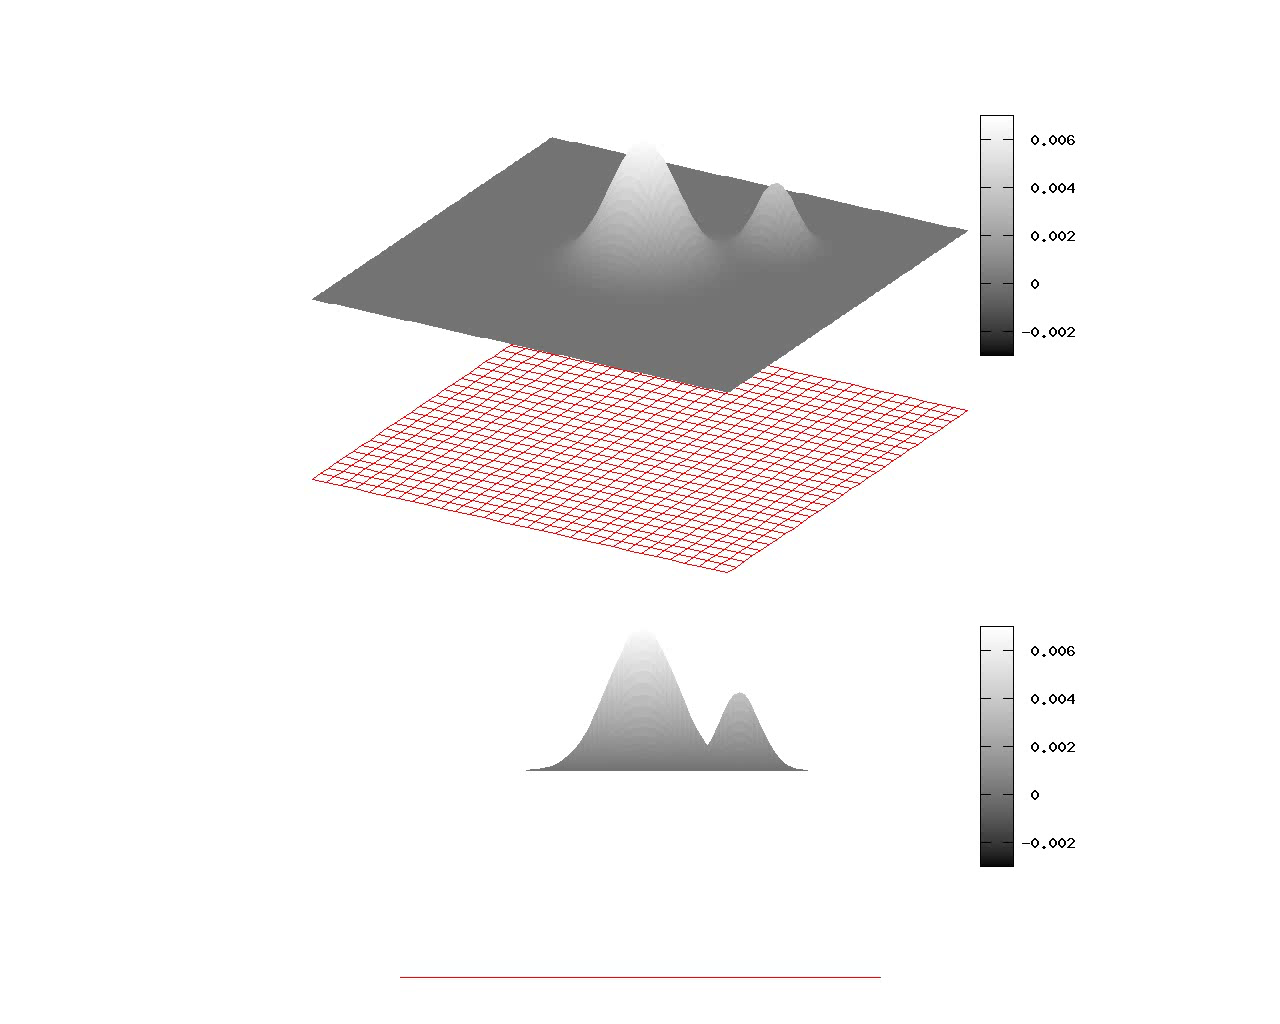
\includegraphics[width=8cm]{complex_drop1.png}
    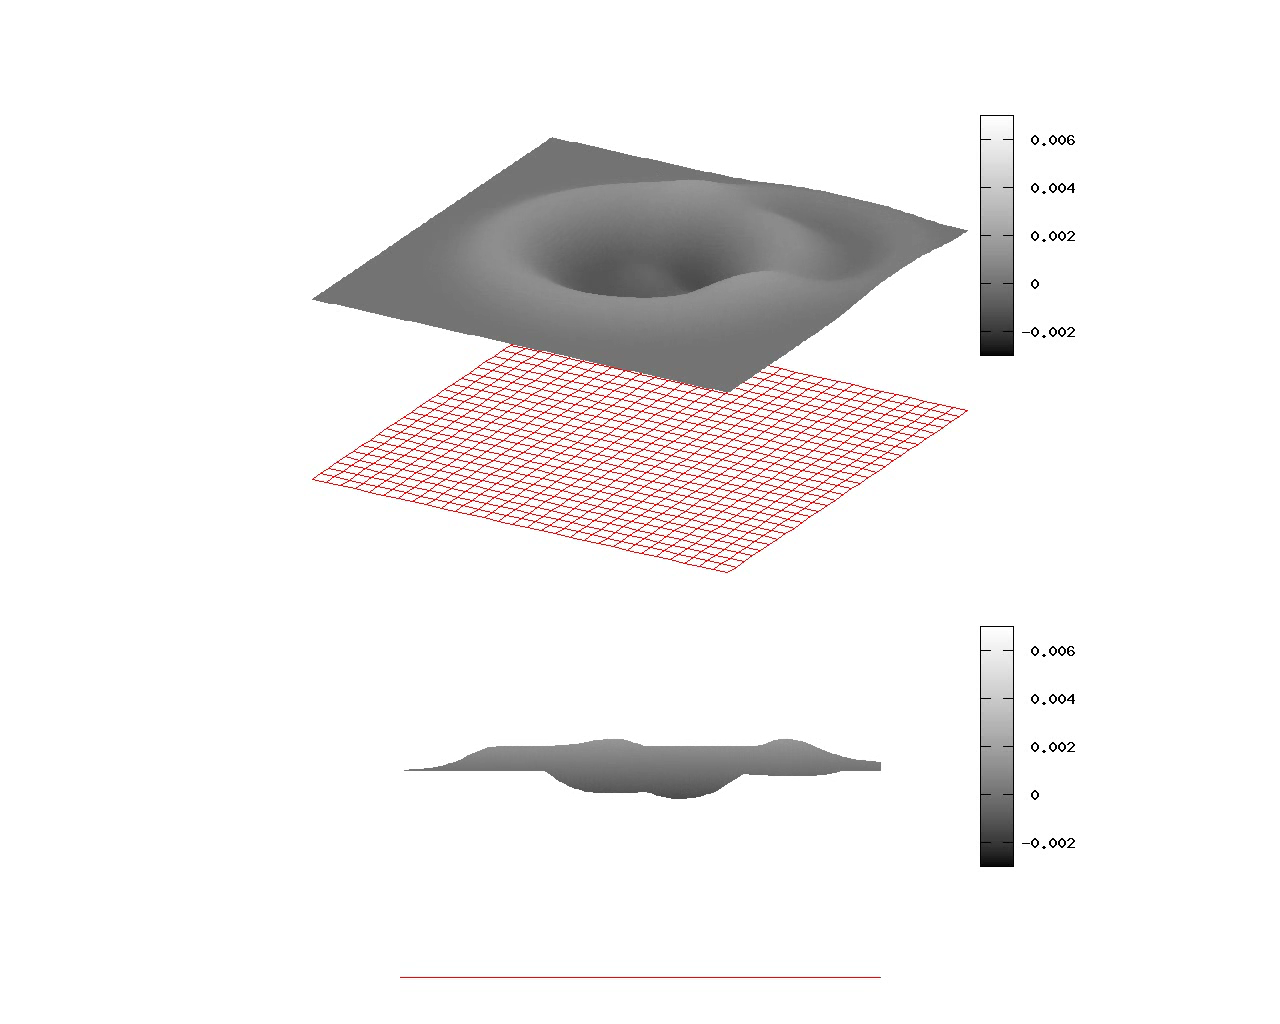
\includegraphics[width=8cm]{complex_drop2.png}
    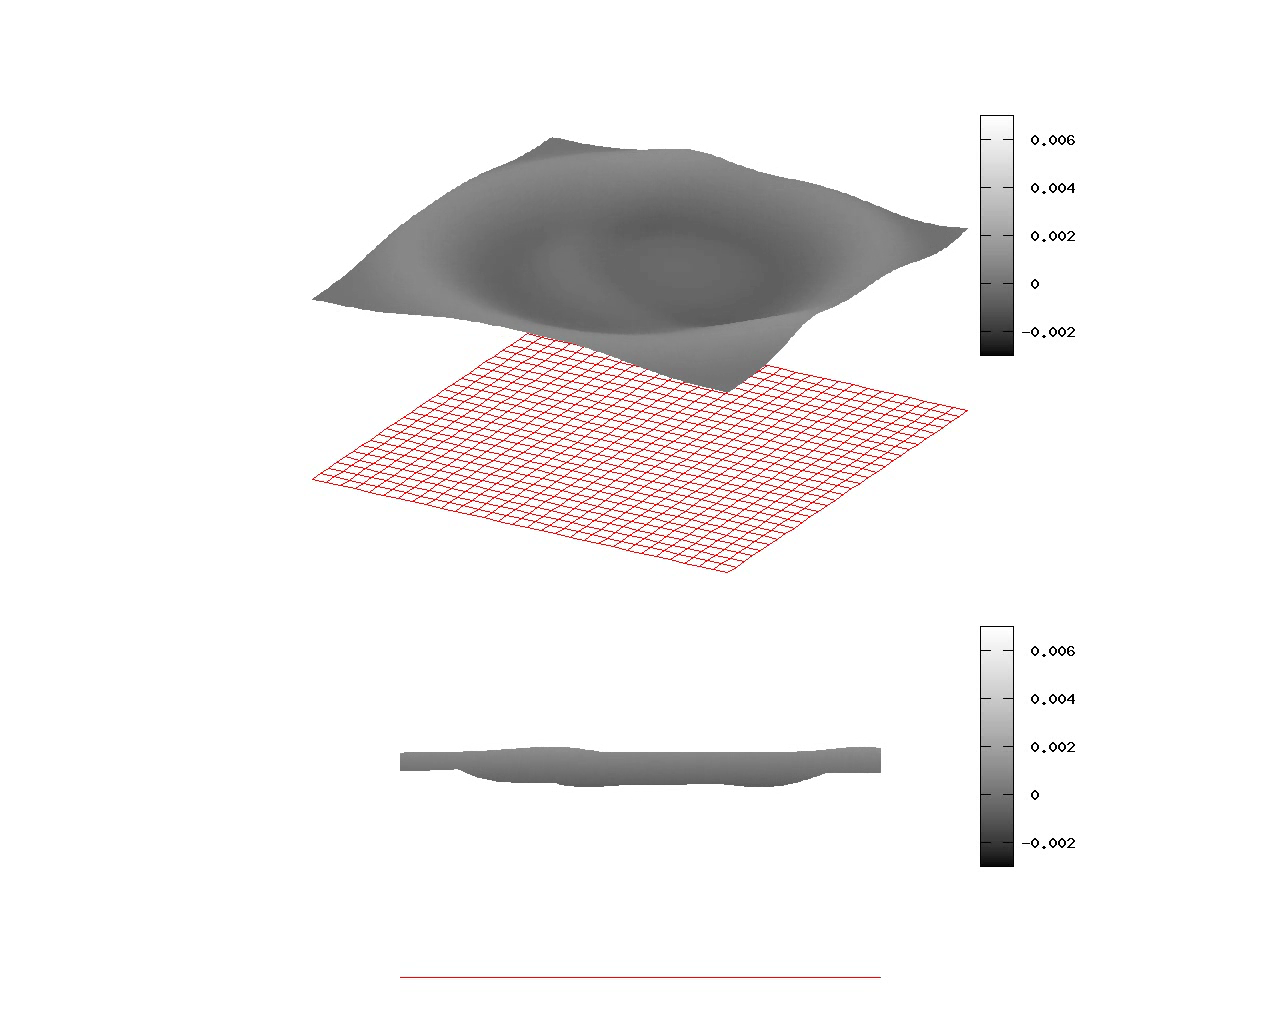
\includegraphics[width=8cm]{complex_drop3.png}
    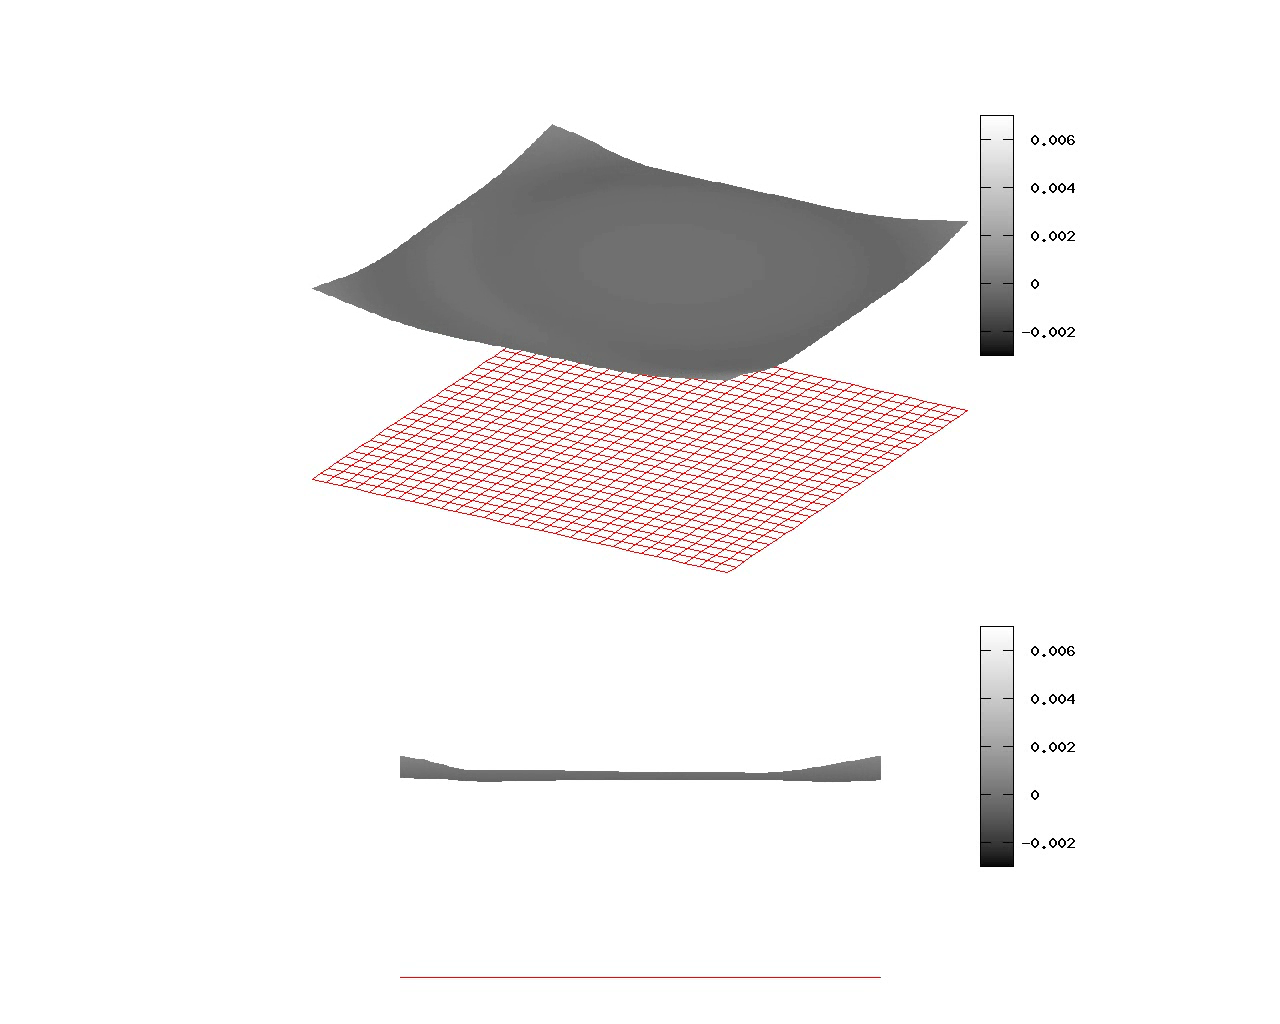
\includegraphics[width=8cm]{complex_drop4.png}
    \caption{Результат расчета для нелинейной системы($F_{nonlin}\neq 0$) со сложной начальной формой на нулевом, 80, 180 и 280 шаге}
    \label{fig:ComplexDrop}
\end{figure}

\newpage
Рассмотрим задачу о движении начальной волны следующего вида:

$u_0=0\;v_0=0\;\eta_0=4 \cdot 10^{-3}e^{-300 ((x-0.3)^2)}+4 \cdot 10^{-3}e^{(-300 ((x-0.7)^2+(y-0.7)^2))}$

в единичном квадрате глубиной $H(x,y)=10^{-2}$.

\begin{table}[H]
    \label{tab:FirstResult}
    \caption{Параметры для расчета со сложной формой поверхности}
    \begin{center}
	\begin{tabular}{|c|c|c|}
	    \hline
	    Размер области & $1\times1$\\
	    \hline
	    Количество шагов & $300$\\
	    \hline
	    Шаг по времени & $0.01$\\
	    \hline
	    Шаг сетки & $0.01$\\
	    \hline
	    Точность метода & $10^{-7}$\\
	    \hline
	    Форма дна & $H(x,y)=0.01\; B(x,y,t)=0$\\
	    \hline
	\end{tabular}
    \end{center}
\end{table}

На рис.\ref{fig:ComplexDrop2} представлена динамика выхода волны из области решения.

Как видно из представленных расчетов, предлагаемый подход к решению задачи (\ref{eq:MainVectorForm})-(\ref{eq:BoundaryCondition}) позволяет находить в ней решение без отражений или искажений. Волна, движущаяся в расчетной области, проходит через искусственные границы корректно.

\newpage
\begin{figure}[htp]
    \centering
    \vspace{12em}
    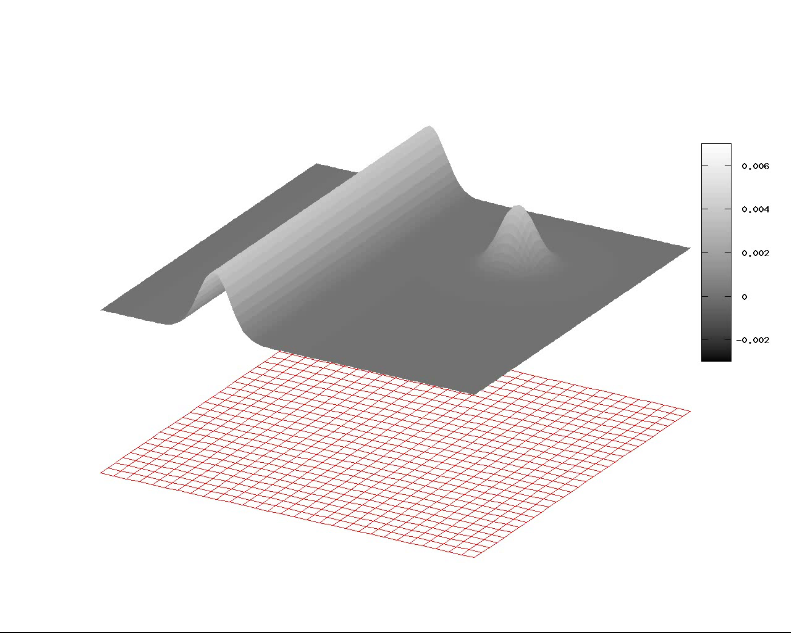
\includegraphics[width=8cm,trim=0 4mm 0 0,clip]{out_nonlin_complex_start21.png}
    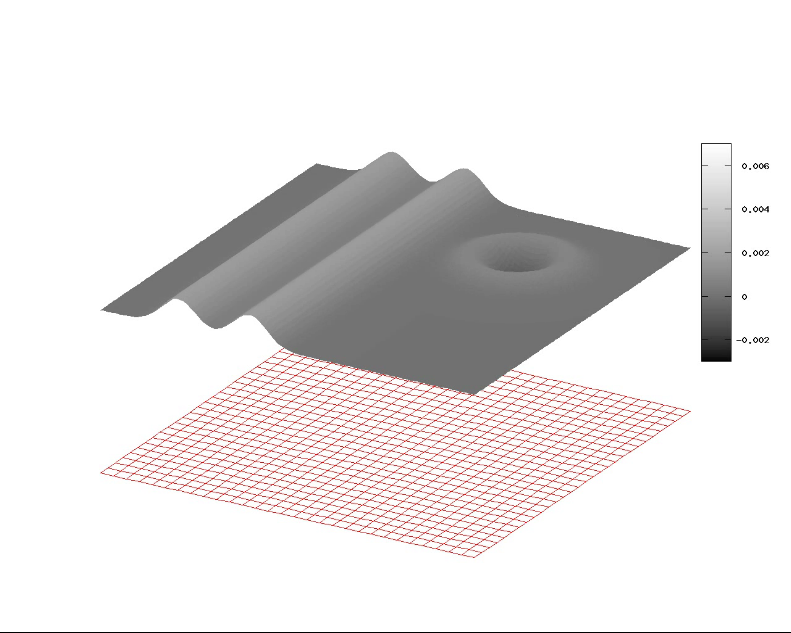
\includegraphics[width=8cm,trim=0 4mm 0 0,clip]{out_nonlin_complex_start22.png}
    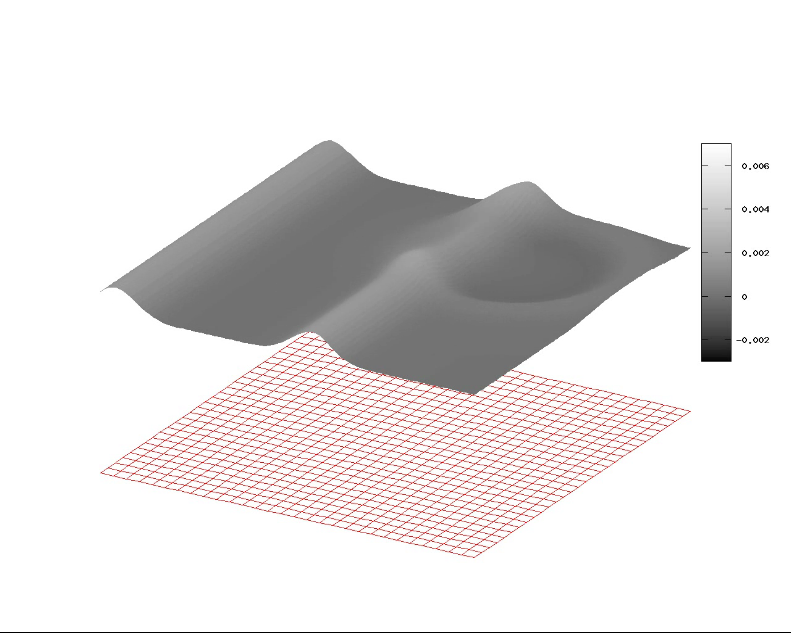
\includegraphics[width=8cm,trim=0 4mm 0 0,clip]{out_nonlin_complex_start23.png}
    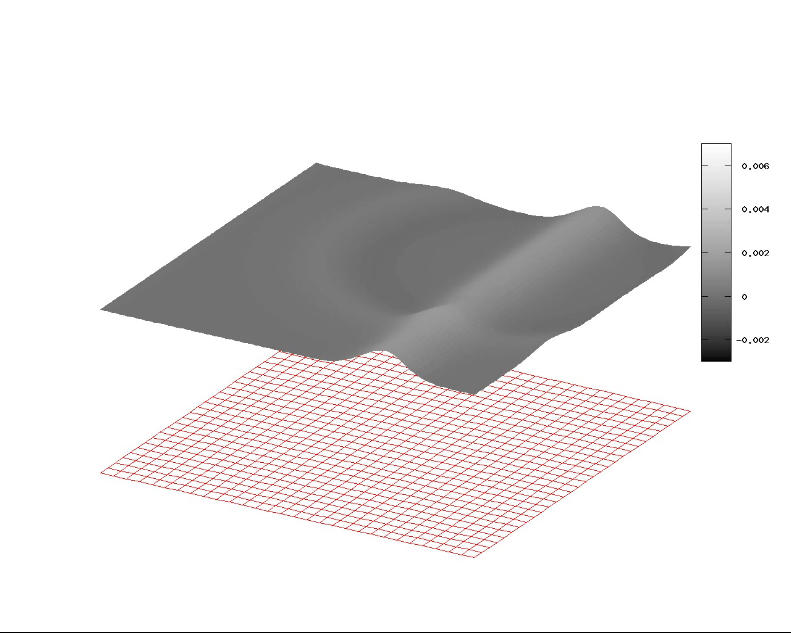
\includegraphics[width=8cm,trim=0 4mm 0 0,clip]{out_nonlin_complex_start24.png}
    \caption{Результат расчета для нелинейной системы($F_{nonlin}\neq 0$) со сложной начальной формой (длинная волна и <<капля>>) на нулевом, 80, 180 и 280 шаге}
    \label{fig:ComplexDrop2}
\end{figure}

\newpage
\addtocounter{section}{1}
\setcounter{equation}{0}
\setcounter{subsection}{0}
\section*{Расчет движения над сложным дном} 
\addtocontents{toc}{\contentsline{section}{\protect\numberline{\S\;\thesection.}\vspace{10pt}Расчет движения над сложным дном}{\thepage}}

Рассмотрим задачу о движении начальной волны следующего вида:

$u_0=0\;v_0=0\;\eta_0=4 \cdot 10^{-3}e^{(-100 (x-0.7)^2)}$

в единичном квадрате глубиной $H(x,y)=10^{-2}$.

\begin{table}[H]
    \label{tab:FirstResult}
    \caption{Параметры для расчета с коническим выступом}
    \begin{center}
	\begin{tabular}{|c|c|c|}
	    \hline
	    Размер области & $1\times1$\\
	    \hline
	    Количество шагов & $1200$\\
	    \hline
	    Шаг по времени & $0.001$\\
	    \hline
	    Шаг сетки & $0.01$\\
	    \hline
	    Точность метода & $10^{-6}$\\
	    \hline
	    Форма дна & $H(x,y)=0.01, \sqrt{(x-5)^2+(y-0.5)^2}>0.05$\\ 
	    & $H(x,y)=0.005, \sqrt{(x-5)^2+(y-0.5)^2}<0.05$\\
	    & $B(x,y,t)=0$\\
	    \hline
	\end{tabular}
    \end{center}
\end{table}

На рис.\ref{fig:CylinderBottom} представлена динамика выхода волны из области решения в двух проекциях для каждого шага.

На рис.\ref{fig:CylinderBottomMap} представлен тот же расчет в проекции свеху.

Видно, что волна, наталкиваясь на препятствие, замедляется в центре, откуда затем по поверхности начинают распространяться колебания.

\newpage
\begin{figure}[htp]
    \centering
    \vspace{12em}
    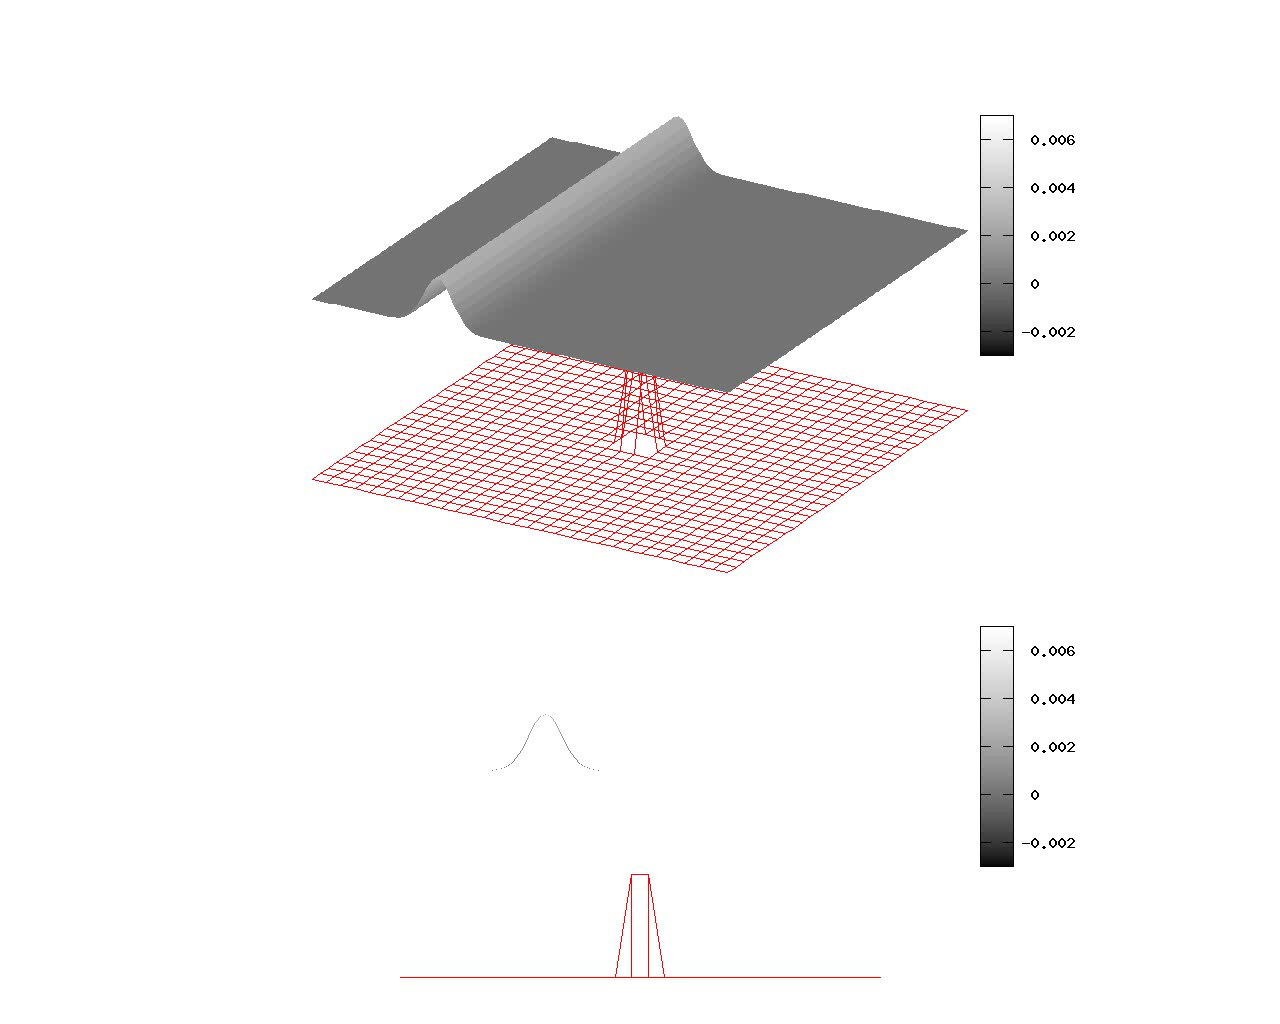
\includegraphics[width=8cm]{cylinder_bottom1.png}
    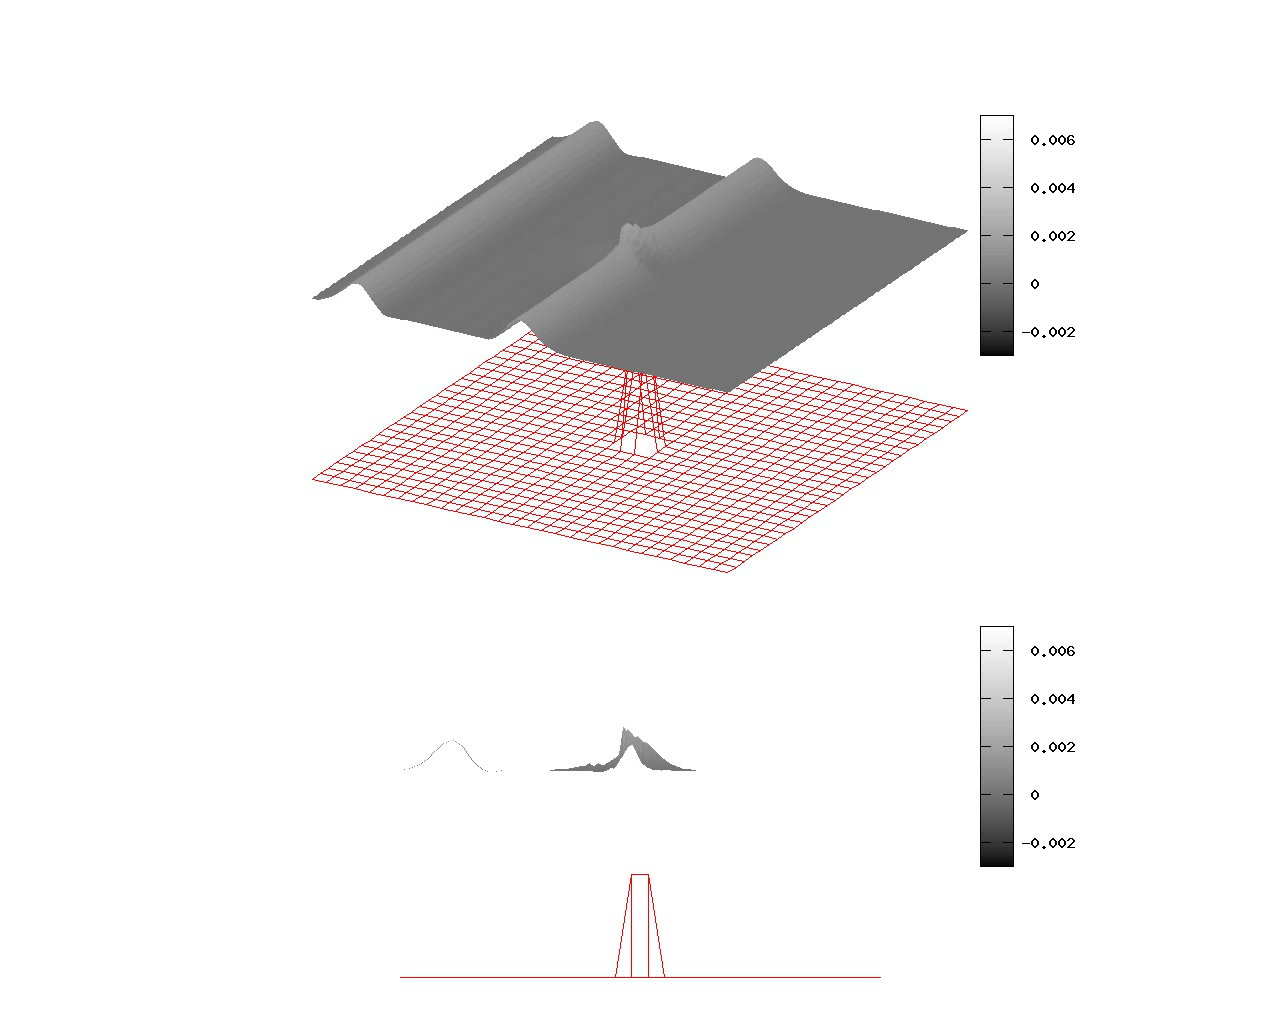
\includegraphics[width=8cm]{cylinder_bottom2.png}
    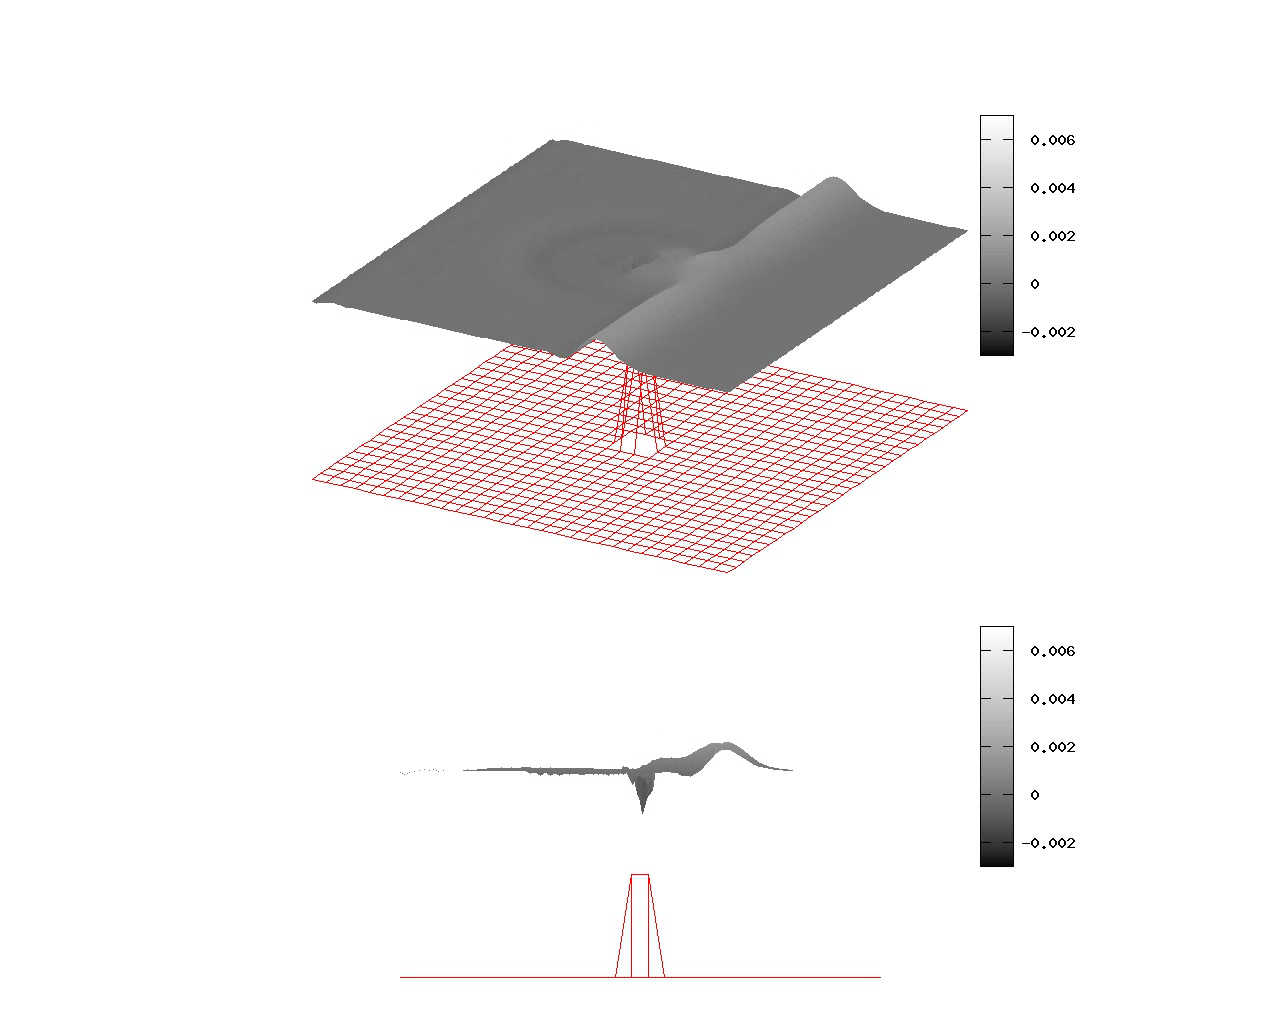
\includegraphics[width=8cm]{cylinder_bottom3.png}
    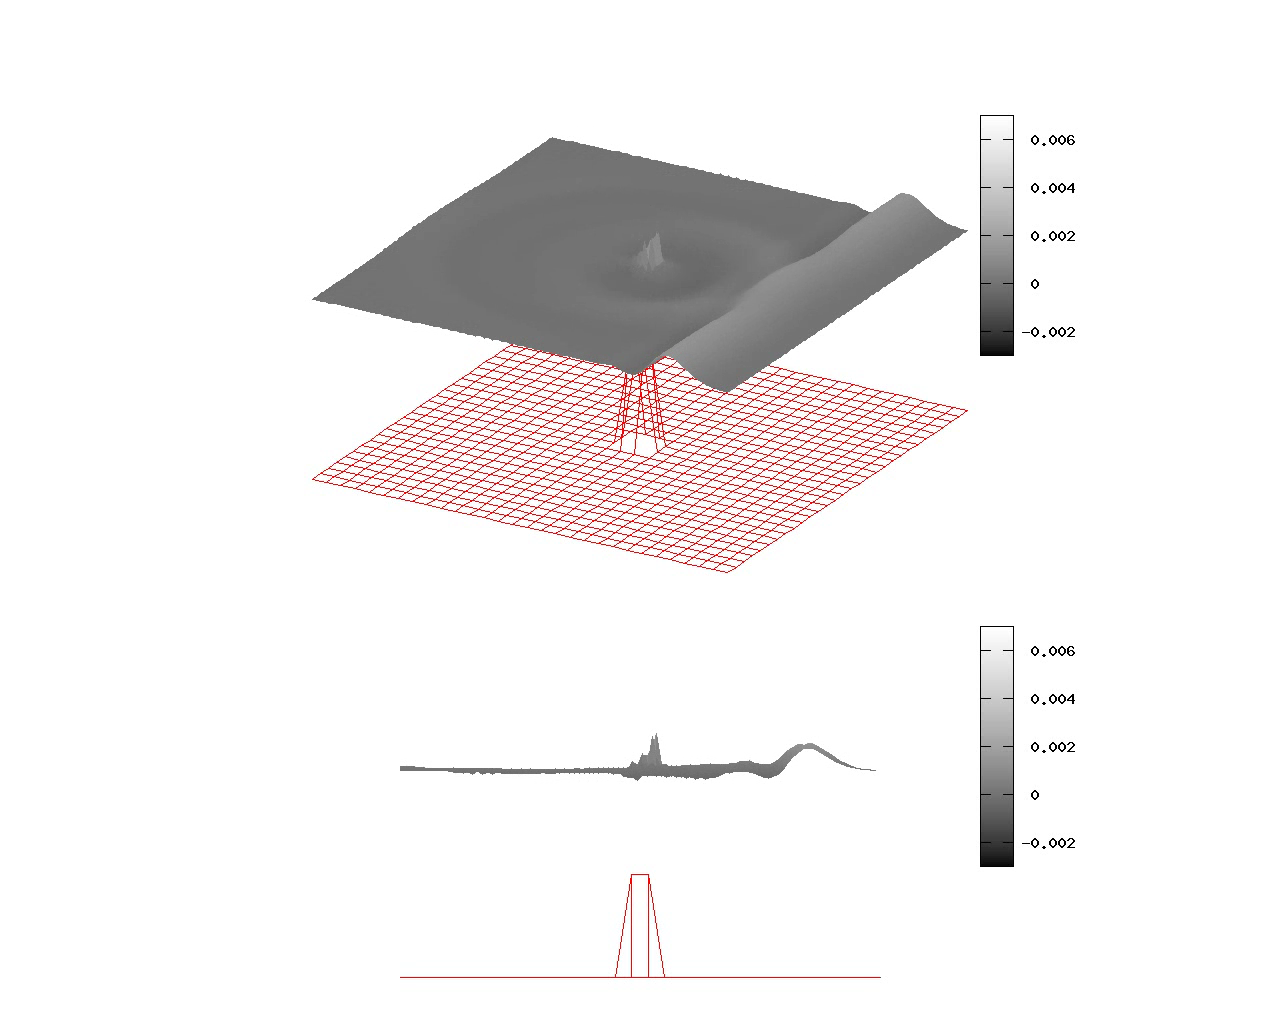
\includegraphics[width=8cm]{cylinder_bottom4.png}
    \caption{Результат расчета для нелинейной системы($F_{nonlin}\neq 0$) с коническим выступом дна на нулевом, 400, 800 и 1200 шаге}
    \label{fig:CylinderBottom}
\end{figure}

\newpage
\begin{figure}[htp]
    \centering
    \vspace{12em}
    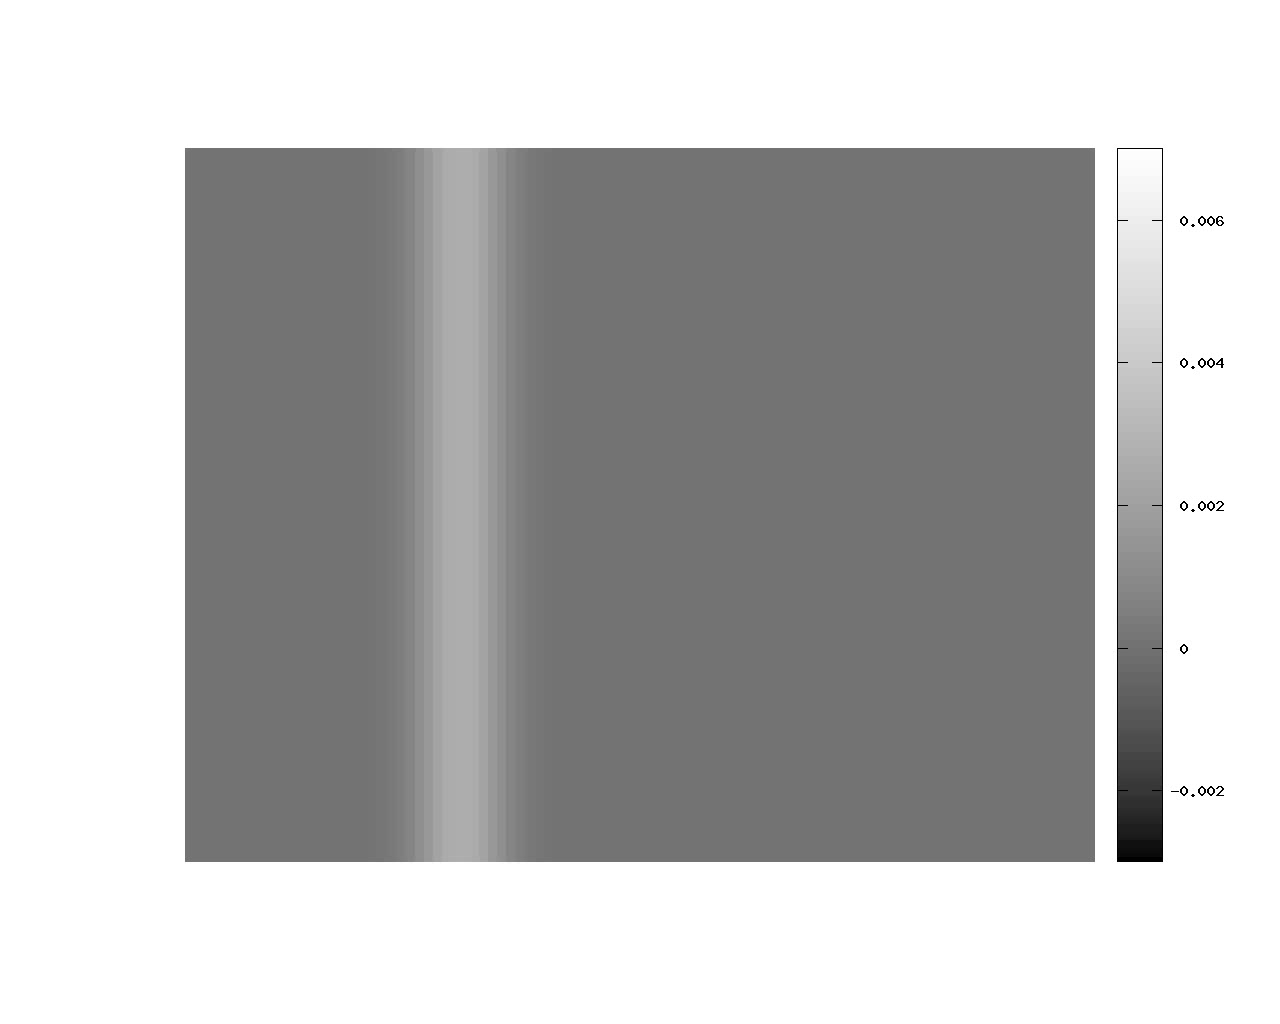
\includegraphics[width=8cm]{cylinder_bottom_map1.png}
    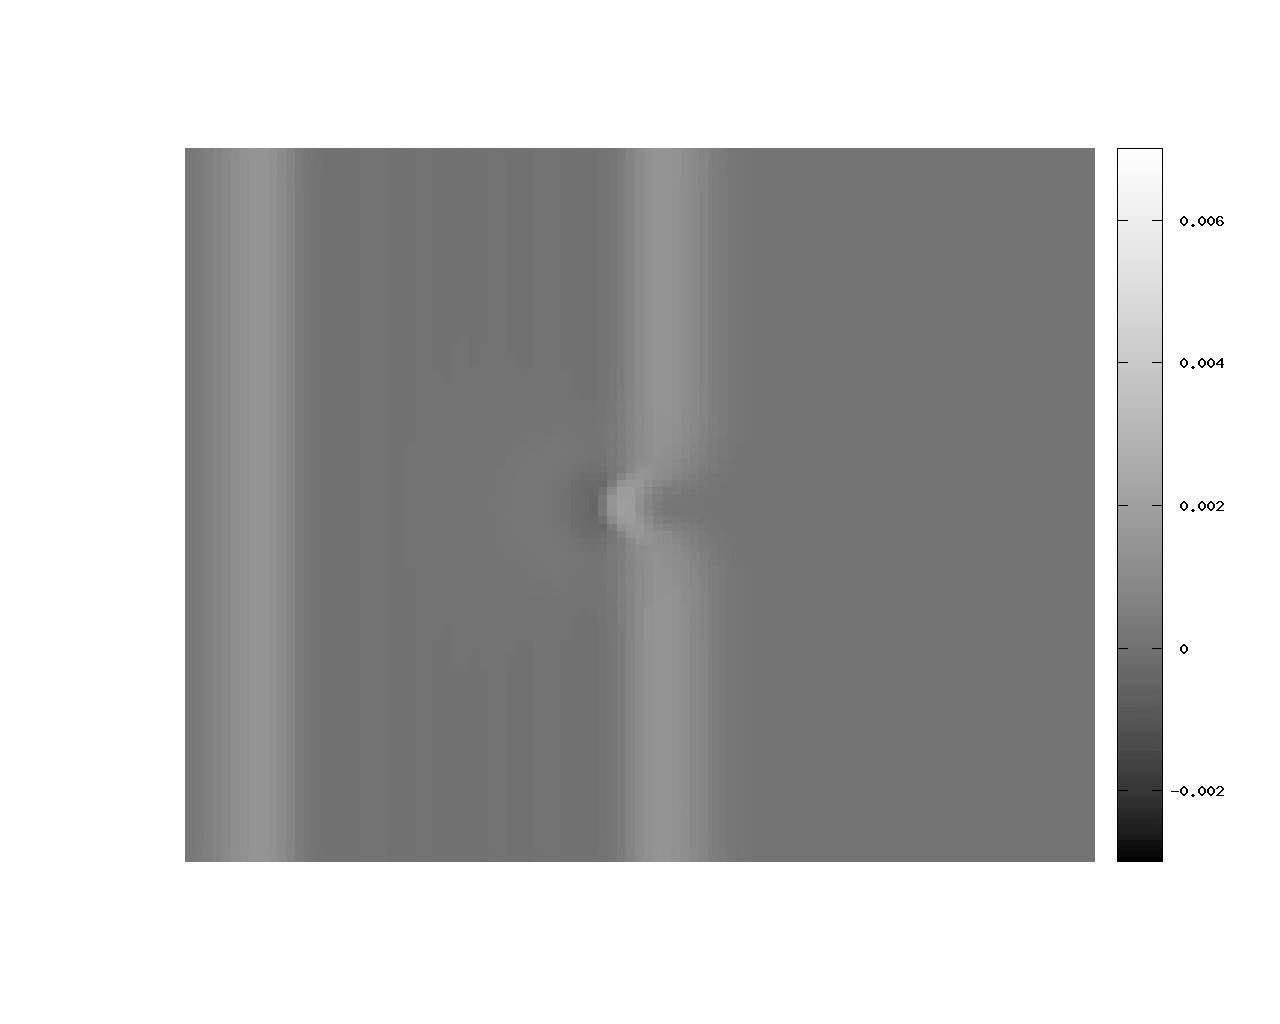
\includegraphics[width=8cm]{cylinder_bottom_map2.png}
    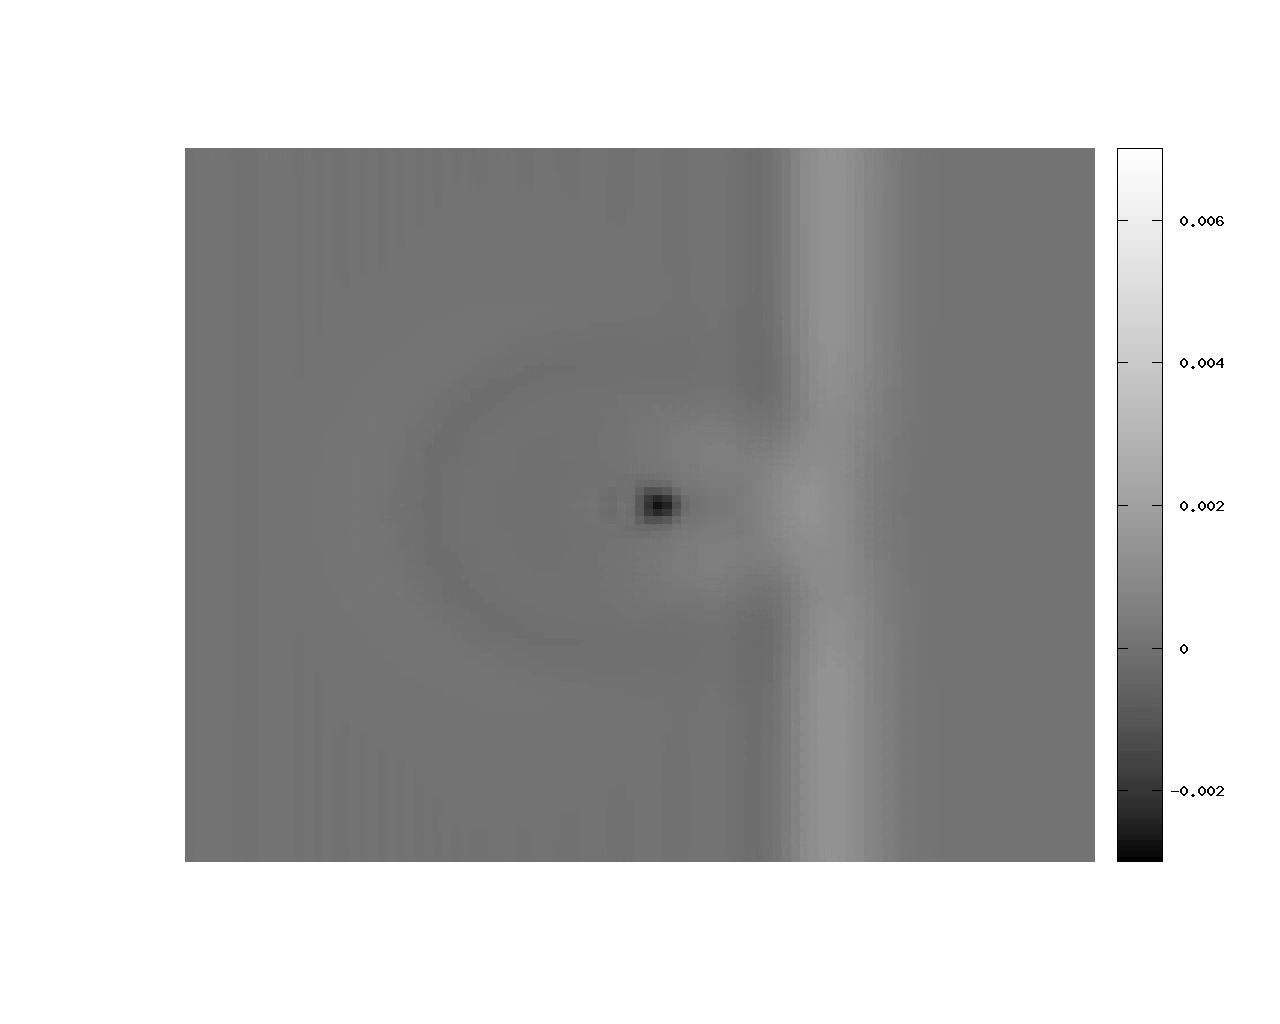
\includegraphics[width=8cm]{cylinder_bottom_map3.png}
    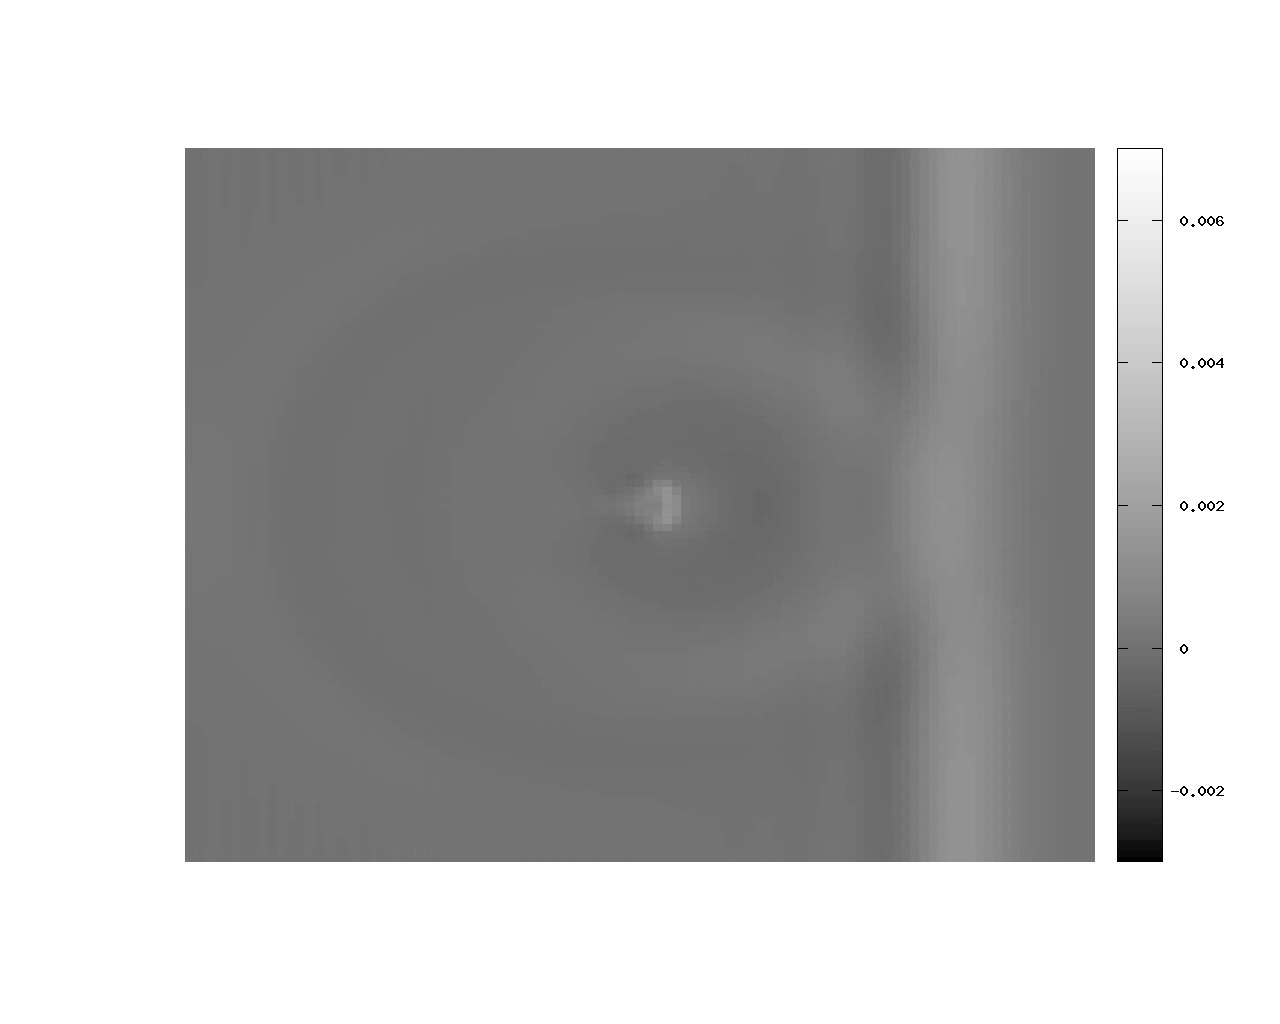
\includegraphics[width=8cm]{cylinder_bottom_map4.png}
    \caption{Результат расчета для нелинейной системы($F_{nonlin}\neq 0$) с коническим выступом дна на нулевом, 400, 800 и 1200 шаге (проекция сверху)}
    \label{fig:CylinderBottomMap}
\end{figure}

\newpage
Рассмотрим задачу о движении начальной волны следующего вида:

$u_0=0\;v_0=0\;\eta_0=7 \cdot 10^{-3}e^{(-100 (x-0.7)^2)}$

в единичном квадрате глубиной $H(x,y)=10^{-2}$.

\begin{table}[H]
    \label{tab:FirstResult}
    \caption{Параметры для расчета с экспоненциальным выступом}
    \begin{center}
	\begin{tabular}{|c|c|c|}
	    \hline
	    Размер области & $1\times1$\\
	    \hline
	    Количество шагов & $300$\\
	    \hline
	    Шаг по времени & $0.001$\\
	    \hline
	    Шаг сетки & $0.01$\\
	    \hline
	    Точность метода & $10^{-7}$\\
	    \hline
	    Форма дна & $H(x,y)=0.01-3 \cdot 10^{-3}e^{(-100 (x-0.7)^2)}$\\
	    & $B(x,y,t)=0$\\
	    \hline
	\end{tabular}
    \end{center}
\end{table}

На рис.\ref{fig:ExpBottom} представлена динамика выхода волны из области решения в двух проекциях для каждого шага.

Из расчетов, представленных в этом параграфе, видно, что предлагаемый подход к решению задачи (\ref{eq:MainVectorForm})-(\ref{eq:BoundaryCondition}) над неровным дном также позволяет находить решение без искажений или отражений. Волна, движущаяся в расчетной области, по-прежнему корректно проходит через искусственные границы, соответствующим образом изменяя свою форму над неровностями дна (например, замедляясь на подъемах).

\newpage
\begin{figure}[htp]
    \centering
    \vspace{12em}
    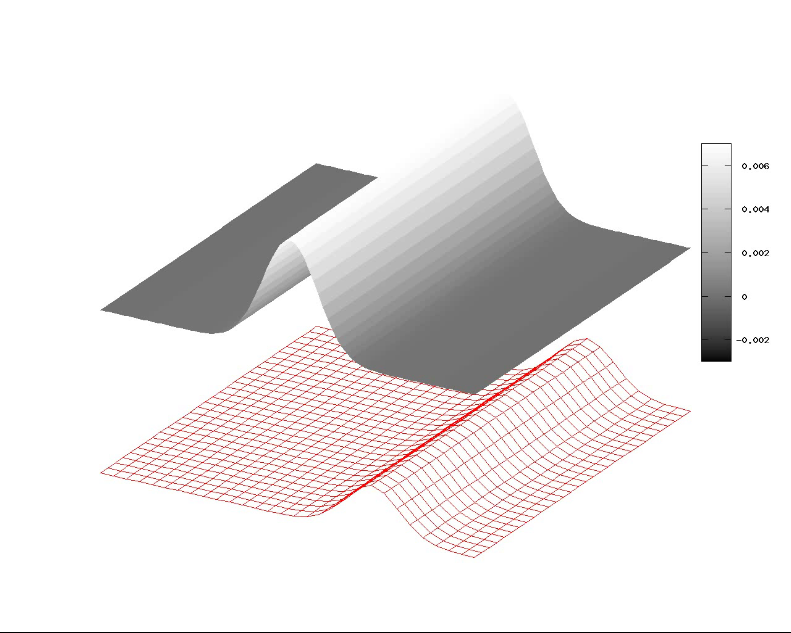
\includegraphics[width=8cm,trim=0 4mm 0 0,clip]{wave_on_exp1.png}
    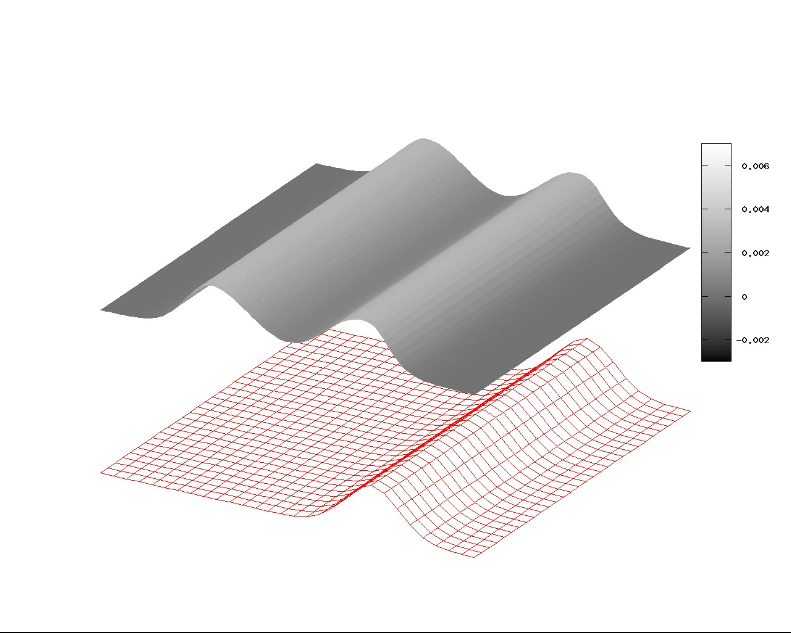
\includegraphics[width=8cm,trim=0 4mm 0 0,clip]{wave_on_exp2.png}
    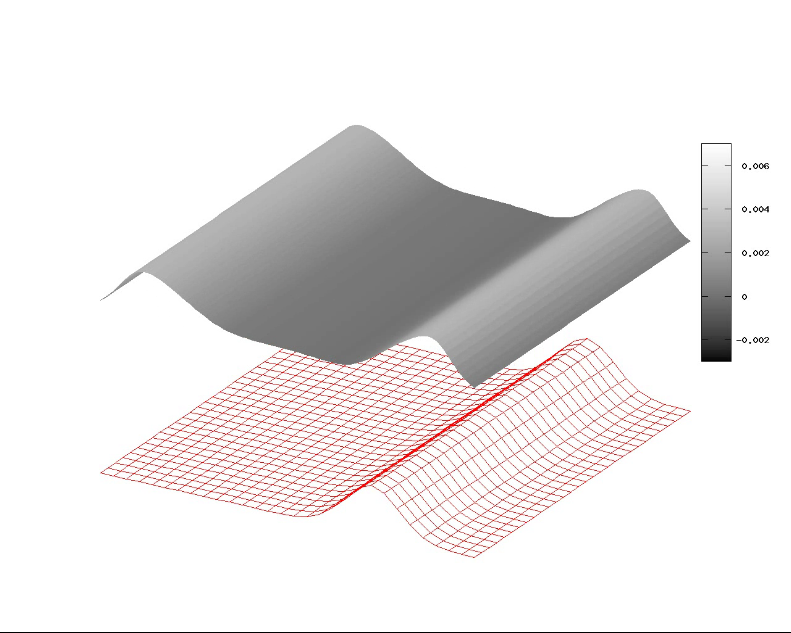
\includegraphics[width=8cm,trim=0 4mm 0 0,clip]{wave_on_exp3.png}
    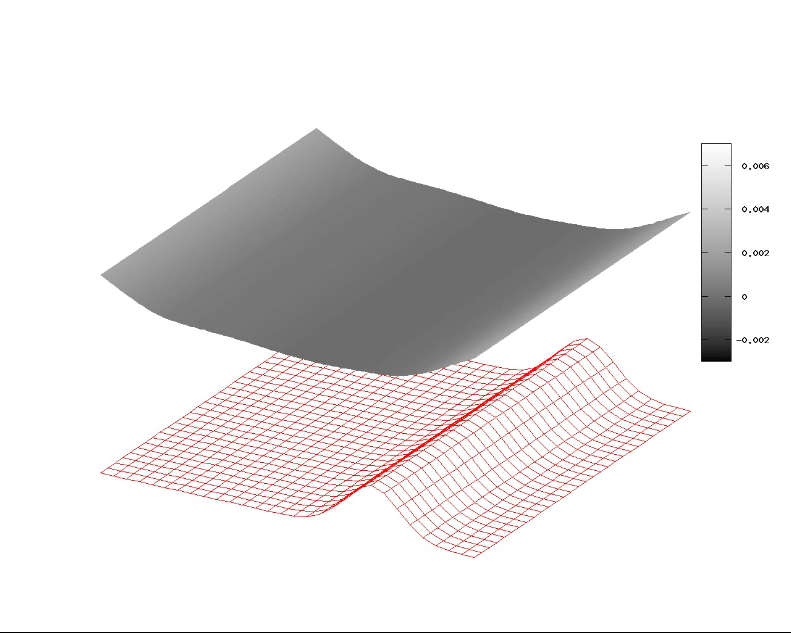
\includegraphics[width=8cm,trim=0 4mm 0 0,clip]{wave_on_exp4.png}
    \caption{Результат расчета для нелинейной системы($F_{nonlin}\neq 0$) с экспоненциальным выступом дна на нулевом, 80, 180 и 280 шаге}
    \label{fig:ExpBottom}
\end{figure}

\newpage
\addtocounter{section}{1}
\setcounter{equation}{0}
\setcounter{subsection}{0}
\section*{Сравнение линейных и нелинейных уравнений} 
\addtocontents{toc}{\contentsline{section}{\protect\numberline{\S\;\thesection.}\vspace{10pt}Сравнение линейных и нелинейных уравнений}{\thepage}}

Рассмотрим задачу о движении начальной волны следующего вида:

$u_0=0\;v_0=0\;\eta_0=7 \cdot 10^{-3}e^{(-100 (x-0.5)^2)}$

в единичном квадрате глубиной $H(x,y)=10^{-2}$.

\begin{table}[H]
    \label{tab:FirstResult}
    \caption{Параметры для расчетов со сравнением линейных и нелинейных уравнений}
    \begin{center}
	\begin{tabular}{|c|c|c|}
	    \hline
	    Размер области & $1\times1$\\
	    \hline
	    Количество шагов & $300$\\
	    \hline
	    Шаг по времени & $0.01$\\
	    \hline
	    Шаг сетки & $0.01$\\
	    \hline
	    Точность метода & $10^{-7}$\\
	    \hline
	    Форма дна & $H(x,y)=0.01\;B(x,y,t)=0$\\
	    \hline
	\end{tabular}
    \end{center}
\end{table}

На рис.\ref{fig:SimpleWaveLin} представлена динамика выхода волны из области решения в случае линейных уравнений.

На рис.\ref{fig:SimpleWaveNonLin} представлена динамика выхода волны из области решения в случае нелинейных уравнений.

На рис.\ref{fig:SimpleWaveDelta} представлена динамика разности этих расчетов.

Заметно, что расчет с нелинейными уравнениями отличается от аналогичного с линейными уравнениями. В линейном случае волна более симметрична относительно своей оси, в нелинейном - форма волны наклоняется в сторону движения.

\newpage
\begin{figure}[htp]
    \centering
    \vspace{12em}
    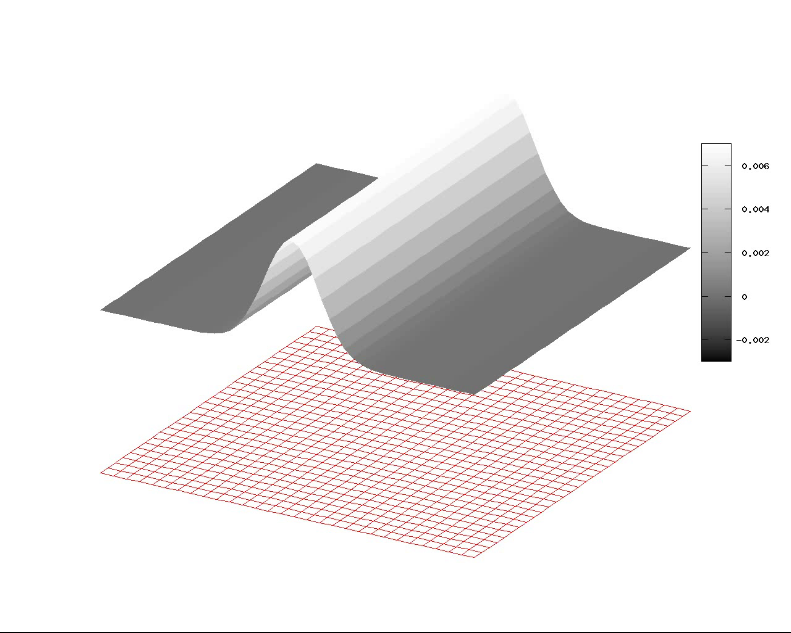
\includegraphics[width=8cm,trim=0 4mm 0 0,clip]{simple_wave_lin1.png}
    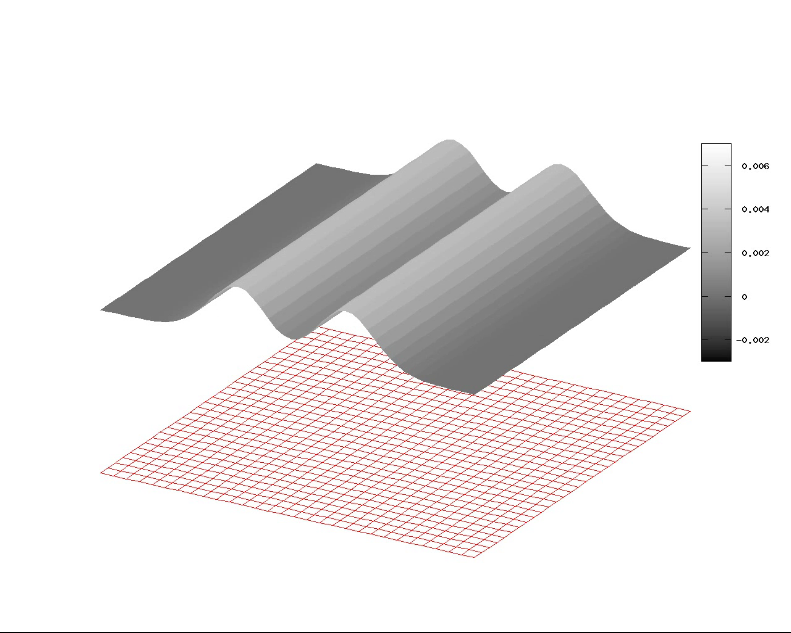
\includegraphics[width=8cm,trim=0 4mm 0 0,clip]{simple_wave_lin2.png}
    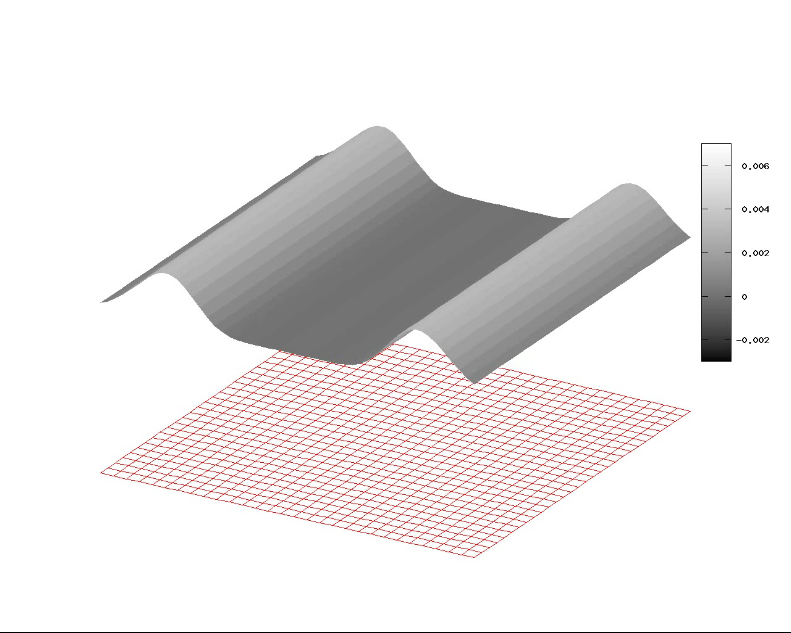
\includegraphics[width=8cm,trim=0 4mm 0 0,clip]{simple_wave_lin3.png}
    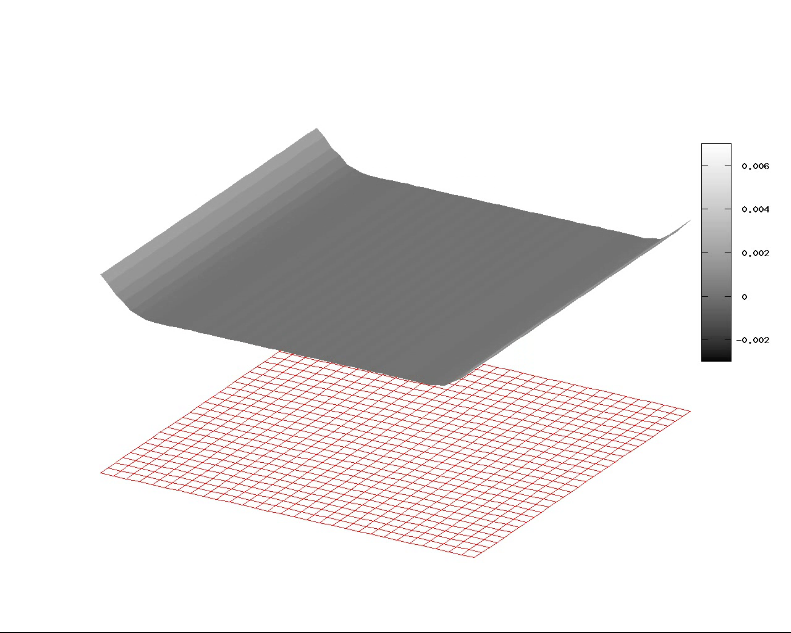
\includegraphics[width=8cm,trim=0 4mm 0 0,clip]{simple_wave_lin4.png}
    \caption{Результат расчета для линейной системы($F_{nonlin}=0$) с ровным дном на нулевом, 80, 180 и 280 шаге}
    \label{fig:SimpleWaveLin}
\end{figure}

\newpage
\begin{figure}[htp]
    \centering
    \vspace{12em}
    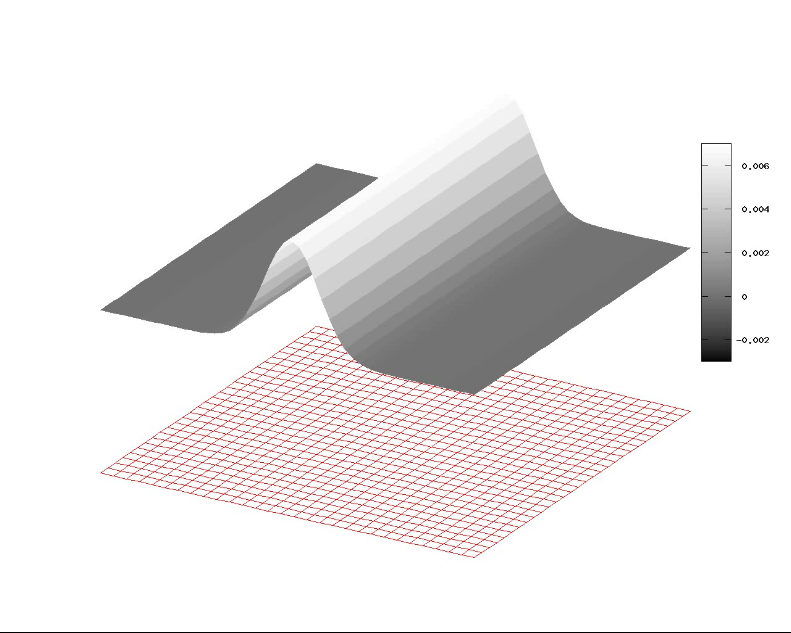
\includegraphics[width=8cm,trim=0 4mm 0 0,clip]{simple_wave_nonlin1.png}
    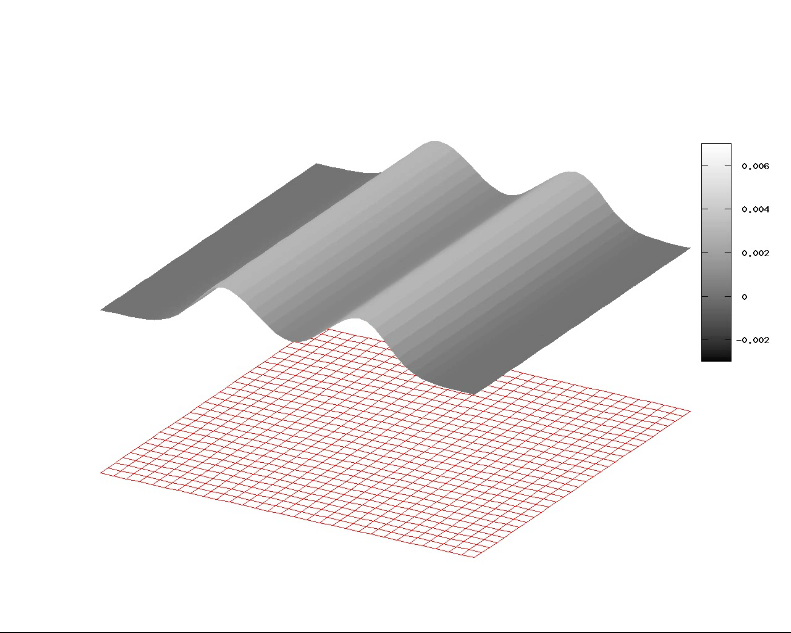
\includegraphics[width=8cm,trim=0 4mm 0 0,clip]{simple_wave_nonlin2.png}
    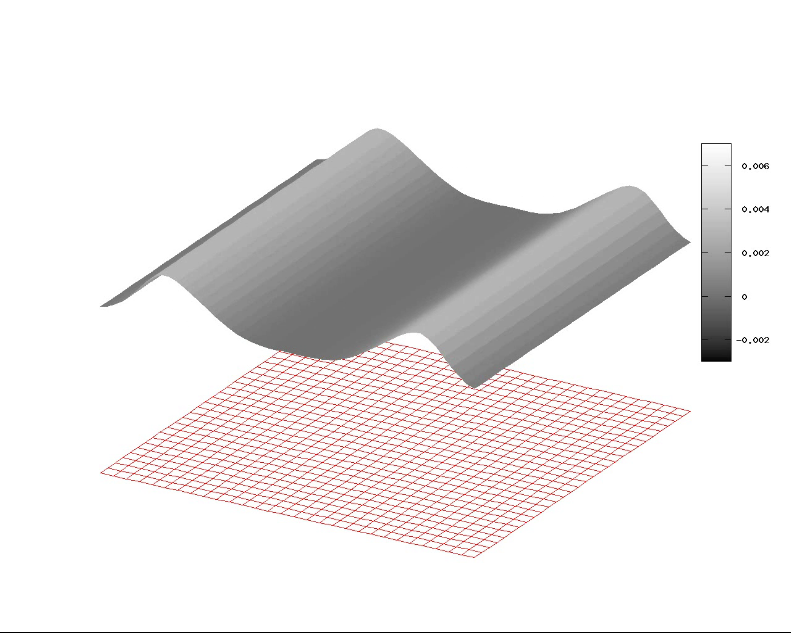
\includegraphics[width=8cm,trim=0 4mm 0 0,clip]{simple_wave_nonlin3.png}
    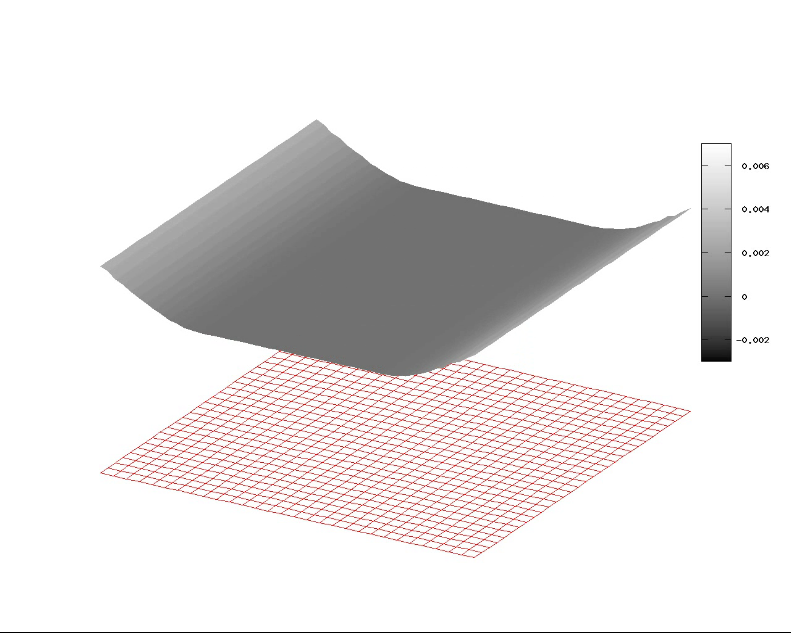
\includegraphics[width=8cm,trim=0 4mm 0 0,clip]{simple_wave_nonlin4.png}
    \caption{Результат расчета для нелинейной системы($F_{nonlin}\neq 0$) с ровным дном на нулевом, 80, 180 и 280 шаге}
    \label{fig:SimpleWaveNonLin}
\end{figure}

\newpage
\begin{figure}[htp]
    \centering
    \vspace{12em}
    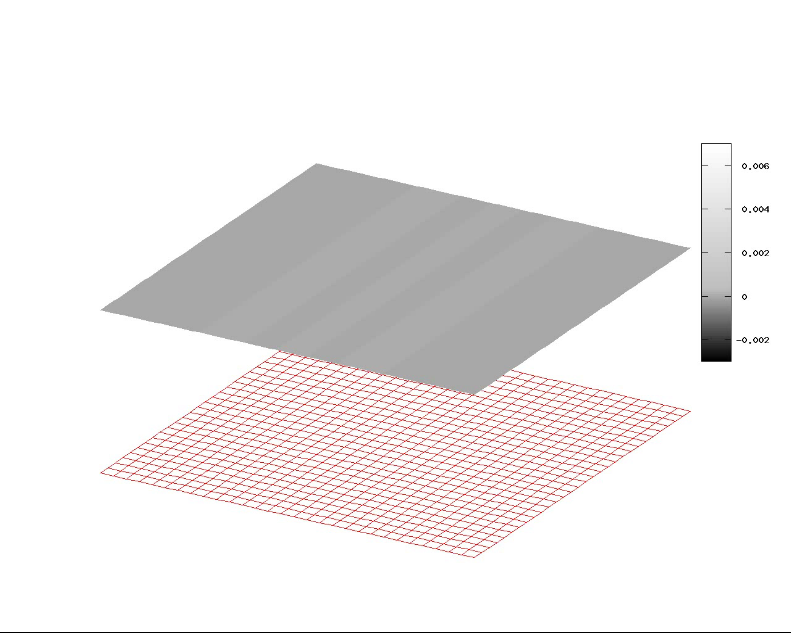
\includegraphics[width=8cm,trim=0 4mm 0 0,clip]{simple_wave_delta1.png}
    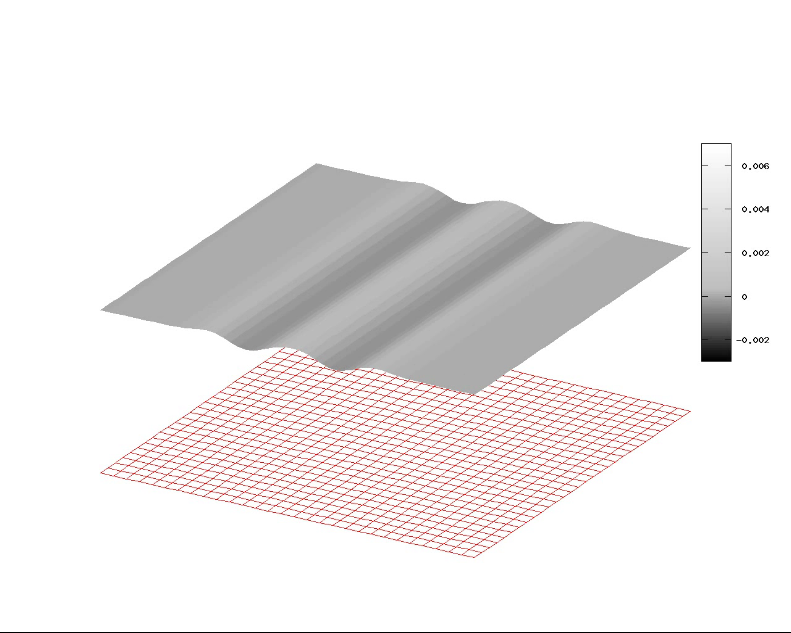
\includegraphics[width=8cm,trim=0 4mm 0 0,clip]{simple_wave_delta2.png}
    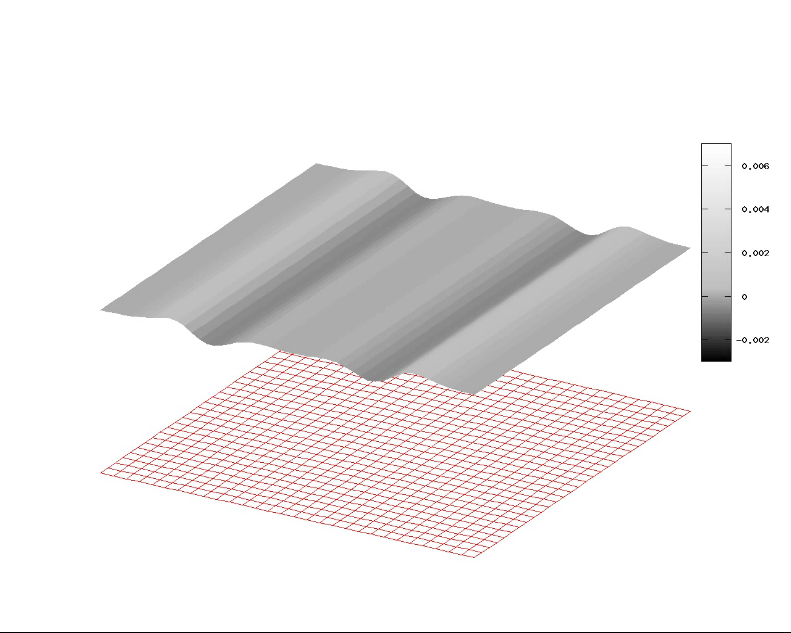
\includegraphics[width=8cm,trim=0 4mm 0 0,clip]{simple_wave_delta3.png}
    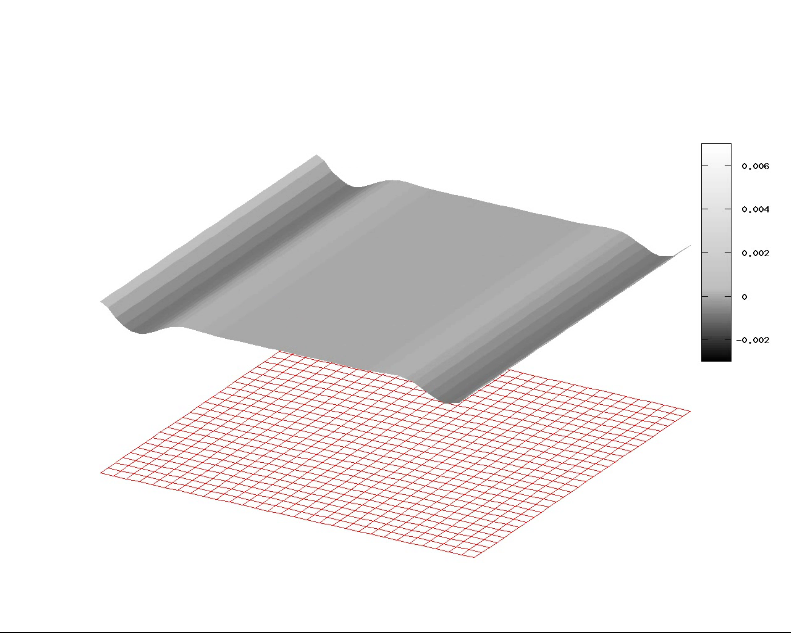
\includegraphics[width=8cm,trim=0 4mm 0 0,clip]{simple_wave_delta4.png}
    \caption{Динамика разности расчетов в линейном и нелинейном случае с ровным дном на нулевом, 80, 180 и 280 шаге}
    \label{fig:SimpleWaveDelta}
\end{figure}

\newpage
Рассмотрим задачу о движении начальной волны следующего вида:

$u_0=0\;v_0=0\;\eta_0=7 \cdot 10^{-3}e^{(-100 (x-0.5)^2)}$

в единичном квадрате глубиной $H(x,y)=10^{-2}$.

\begin{table}[H]
    \label{tab:FirstResult}
    \caption{Параметры для расчетов со сравнением линейных и нелинейных уравнений в случае дна с препятствием на границе}
    \begin{center}
	\begin{tabular}{|c|c|c|}
	    \hline
	    Размер области & $1\times1$\\
	    \hline
	    Количество шагов & $300$\\
	    \hline
	    Шаг по времени & $0.01$\\
	    \hline
	    Шаг сетки & $0.01$\\
	    \hline
	    Точность метода & $10^{-7}$\\
	    \hline
	    Форма дна & $H(x,y)=10^{-2}-3 \cdot 10^{-3}e^{(-100 (x-0.7)^2)}$\\
	    & $B(x,y,t)=0$\\
	    \hline
	\end{tabular}
    \end{center}
\end{table}

На рис.\ref{fig:ExpWaveLin} представлена динамика выхода волны из области решения в случае линейных уравнений.

На рис.\ref{fig:ExpWaveNonLin} представлена динамика выхода волны из области решения в случае нелинейных уравнений.

На рис.\ref{fig:ExpWaveDelta} представлена динамика разности этих расчетов в проекции сверху.

Исходя из представленных расчетов для линейных и нелинейных уравнений, можно отметить, что в нелинейном случае:
\begin{itemize}
    \item Волна со временем меняет свою форму. Она становится немного <<наклоненной>> вперед.
    \item После прохождения основной волны за ней тянется <<хвост>> из небольших колебаний.
    \item С течением времени данные эффекты проявляются более явно.
\end{itemize}

\newpage
\begin{figure}[htp]
    \centering
    \vspace{12em}
    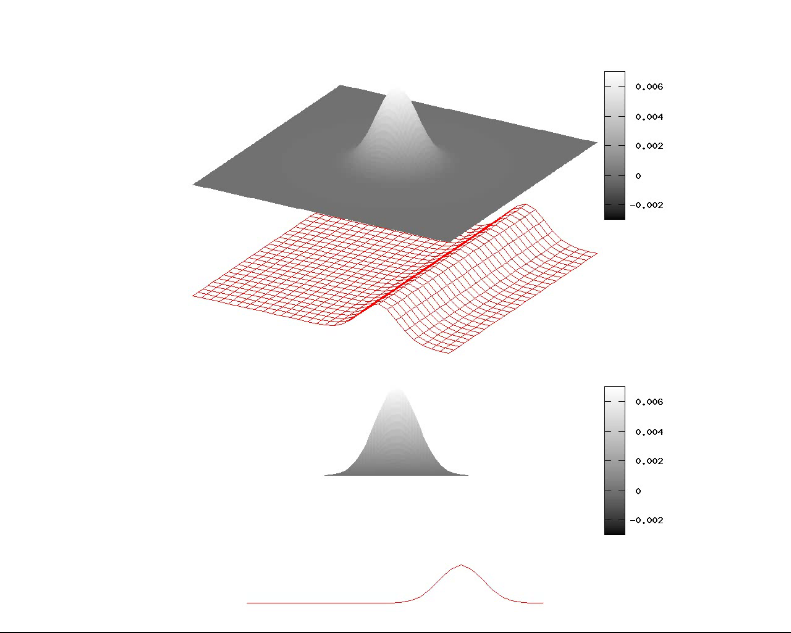
\includegraphics[width=8cm,trim=0 4mm 0 0,clip]{out_lin_drop_exp_bottom1.png}
    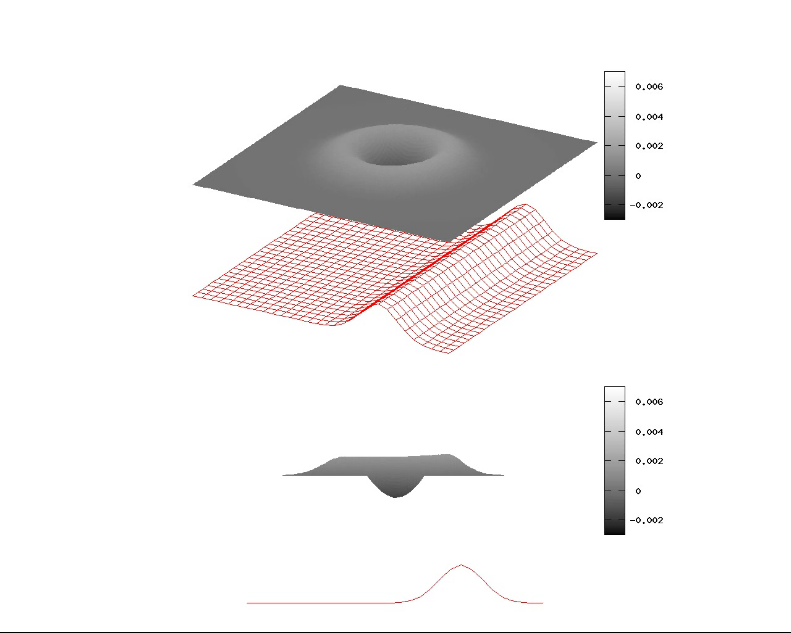
\includegraphics[width=8cm,trim=0 4mm 0 0,clip]{out_lin_drop_exp_bottom2.png}
    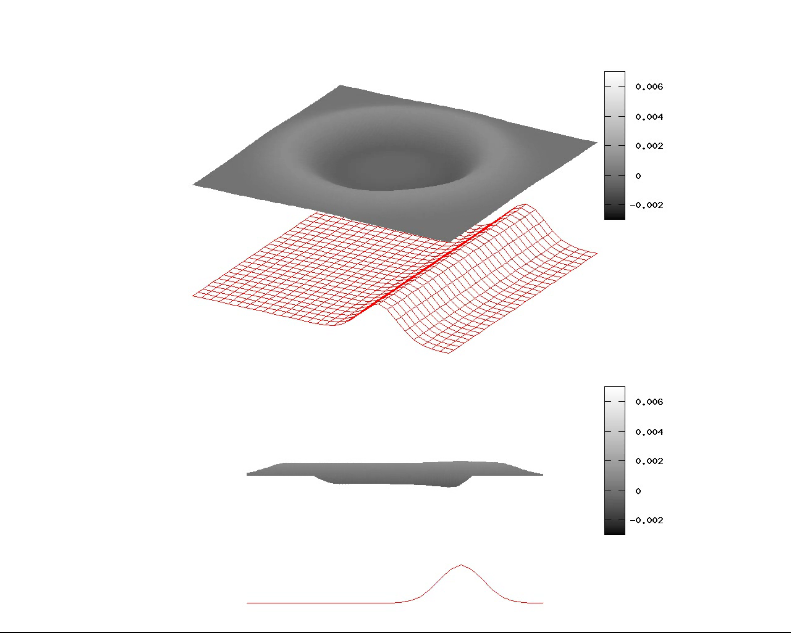
\includegraphics[width=8cm,trim=0 4mm 0 0,clip]{out_lin_drop_exp_bottom3.png}
    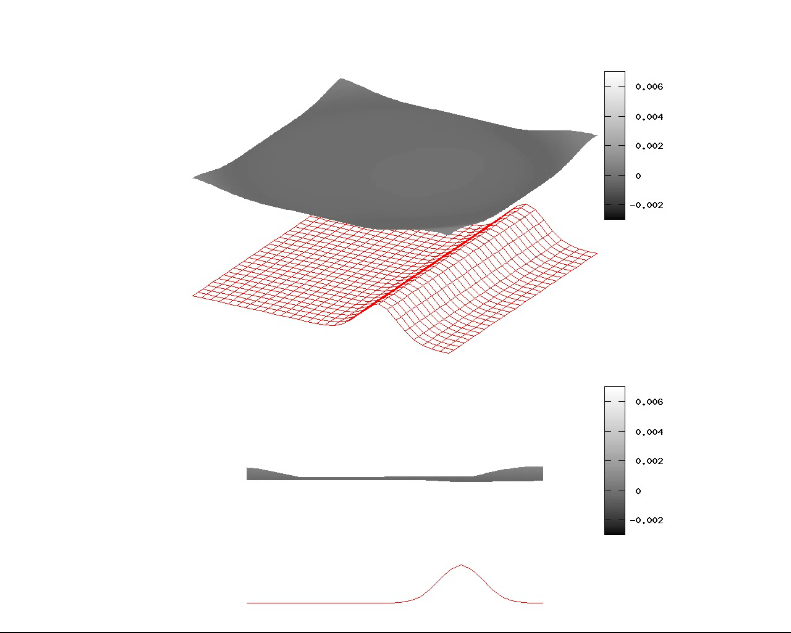
\includegraphics[width=8cm,trim=0 4mm 0 0,clip]{out_lin_drop_exp_bottom4.png}
    \caption{Результат расчета для линейной системы($F_{nonlin}=0$) с препятствием у границы на нулевом, 80, 200 и 380 шаге}
    \label{fig:ExpWaveLin}
\end{figure}

\newpage
\begin{figure}[htp]
    \centering
    \vspace{12em}
    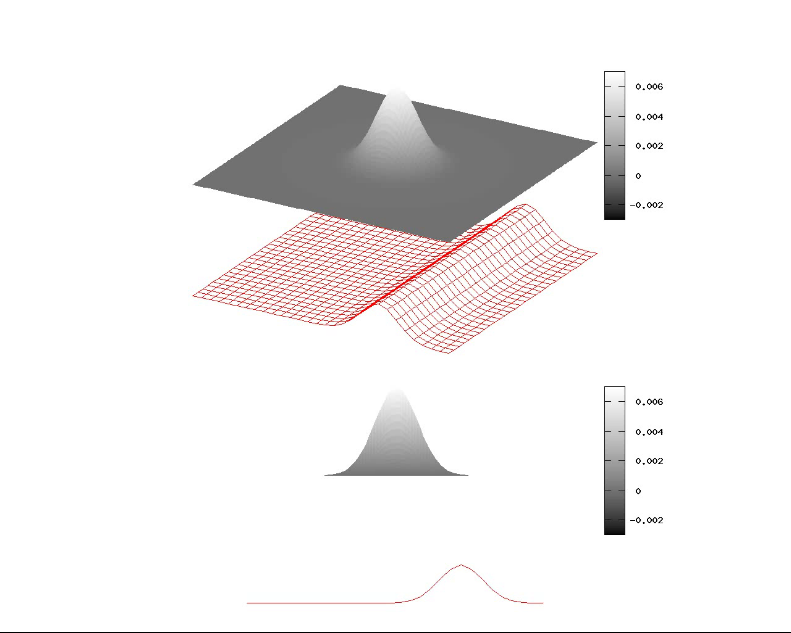
\includegraphics[width=8cm,trim=0 4mm 0 0,clip]{out_nonlin_drop_exp_bottom1.png}
    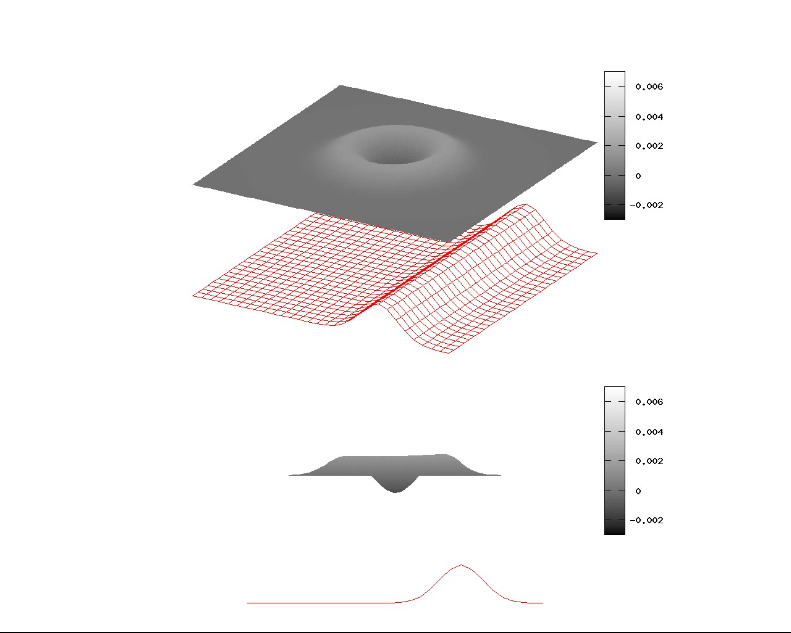
\includegraphics[width=8cm,trim=0 4mm 0 0,clip]{out_nonlin_drop_exp_bottom2.png}
    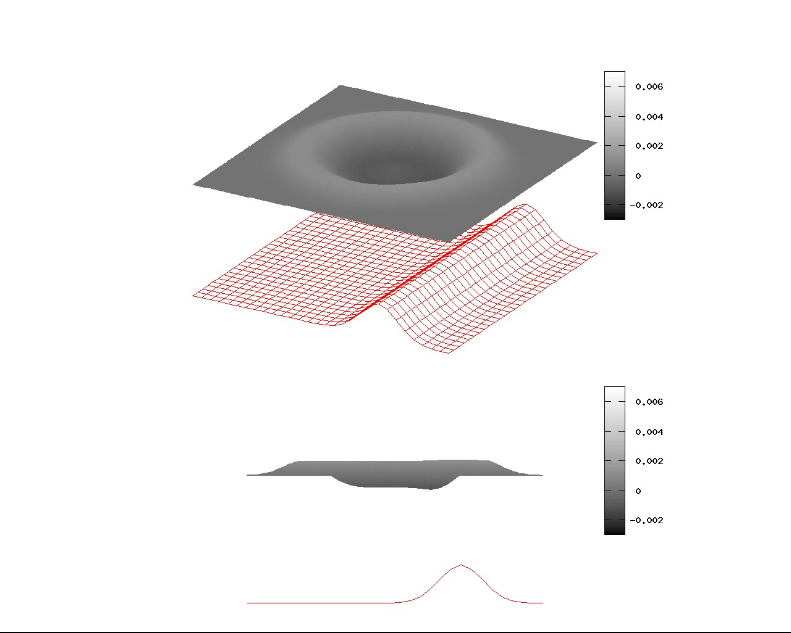
\includegraphics[width=8cm,trim=0 4mm 0 0,clip]{out_nonlin_drop_exp_bottom3.png}
    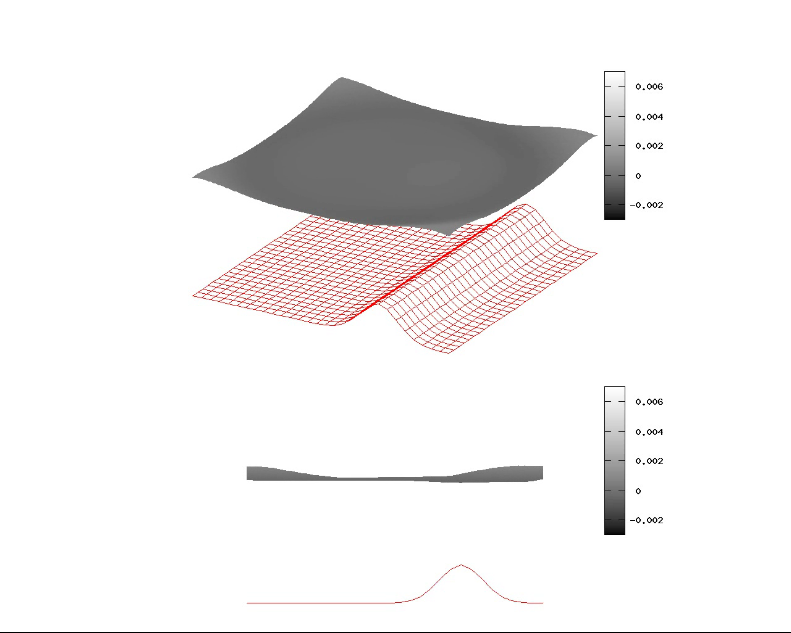
\includegraphics[width=8cm,trim=0 4mm 0 0,clip]{out_nonlin_drop_exp_bottom4.png}
    \caption{Результат расчета для нелинейной системы($F_{nonlin}\neq 0$) с препятствием у границы на нулевом, 80, 200 и 380 шаге}
    \label{fig:ExpWaveNonLin}
\end{figure}

\newpage
\begin{figure}[htp]
    \centering
    \vspace{12em}
    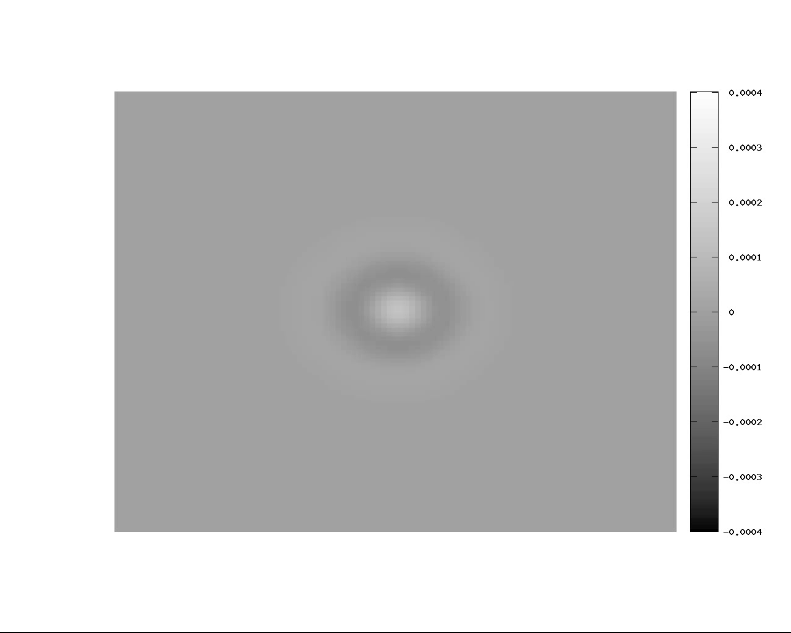
\includegraphics[width=8cm,trim=0 4mm 0 0,clip]{delta_drop_exp_bottom1.png}
    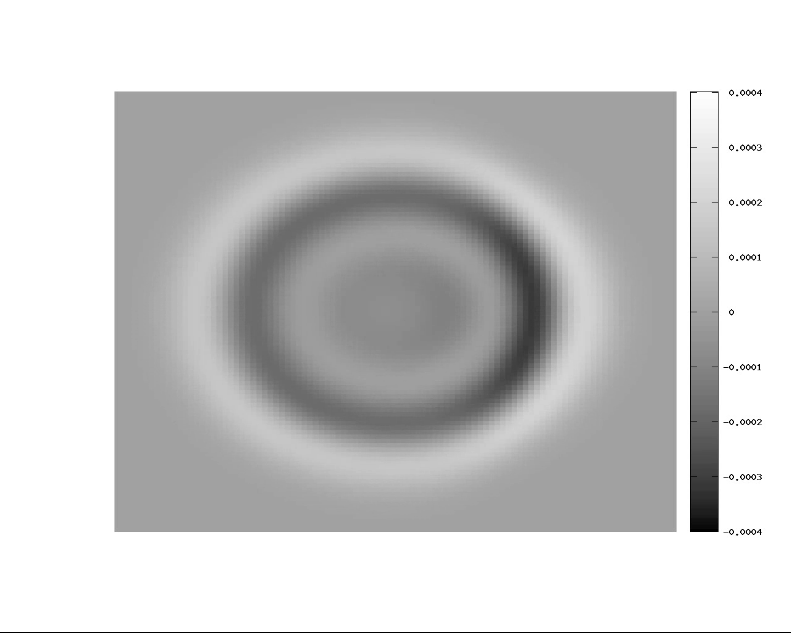
\includegraphics[width=8cm,trim=0 4mm 0 0,clip]{delta_drop_exp_bottom2.png}
    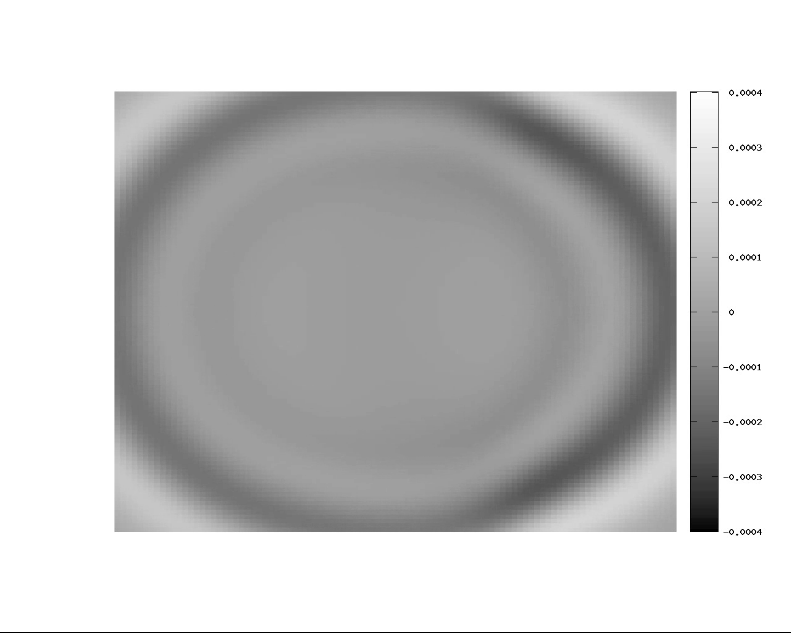
\includegraphics[width=8cm,trim=0 4mm 0 0,clip]{delta_drop_exp_bottom3.png}
    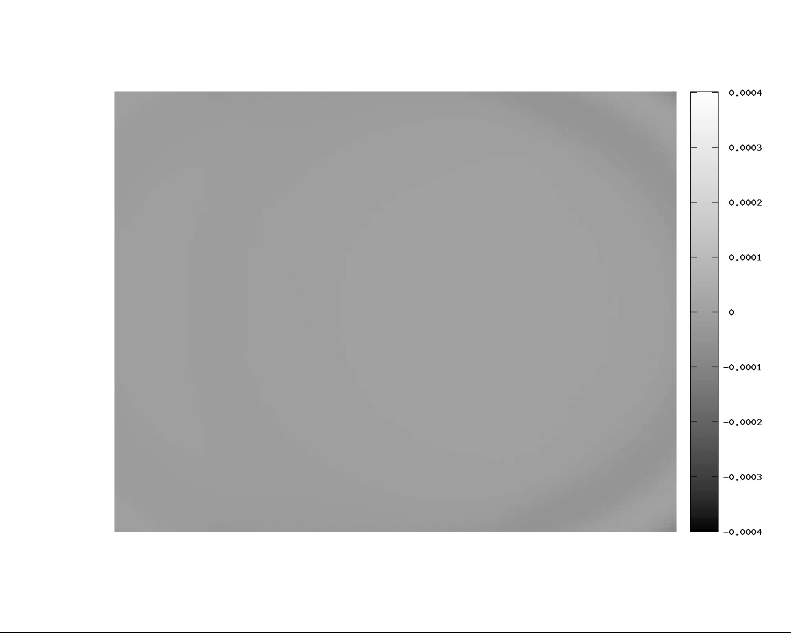
\includegraphics[width=8cm,trim=0 4mm 0 0,clip]{delta_drop_exp_bottom4.png}
    \caption{Динамика разности расчетов в линейном и нелинейном случае с препятствием у границы на 20, 80, 200 и 380 шаге}
    \label{fig:ExpWaveDelta}
\end{figure}

\newpage
\addtocounter{section}{1}
\setcounter{subsection}{0}
\setcounter{equation}{0}
\section*{Эффект возникновения волны}
\addtocontents{toc}{\contentsline{section}{\protect\numberline{\S\;\thesection.}\vspace{10pt}Эффект возникновения волны}{\thepage}}

В процессе проведения расчетов был обнаружен любопытный эффект, который ранее нигде встречался. Данный эффект достаточно устойчив, для того, чтобы не списать его на ошибки или неточности, поэтому привлек внимание.

После того как волна полностью выходит из расчетной области, в ней остаются некоторые регулярные колебания, волны, амплитуда которых меньше, чем исходная. Если продолжить расчет в этой ситуации, либо взять указанные колебания в качестве начальных данных для нового расчета, то произойдет <<возвращение>> волны - т.е. свободная поверхность начинает изменяться и принимает форму, обратную той, что была задана в качестве начального положения.

\begin{figure}[H]
    \centering
    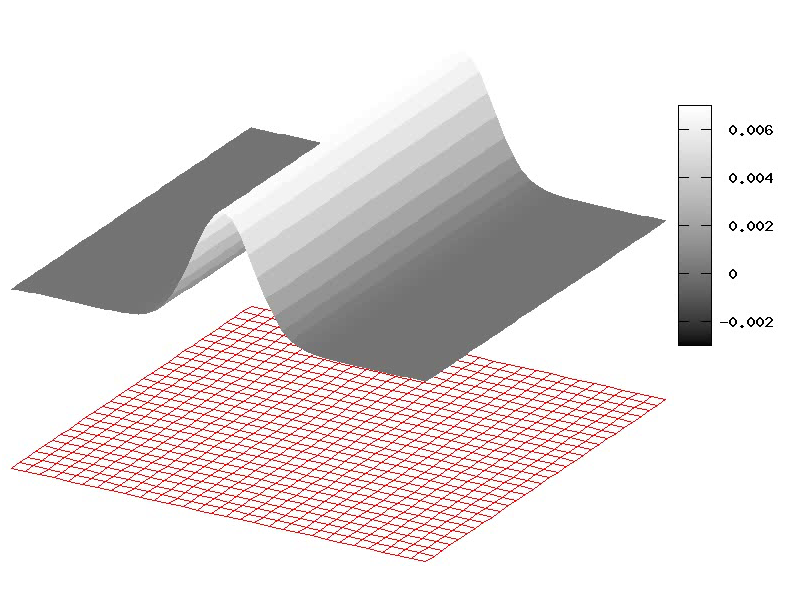
\includegraphics[width=8cm]{simple_return1.png}
    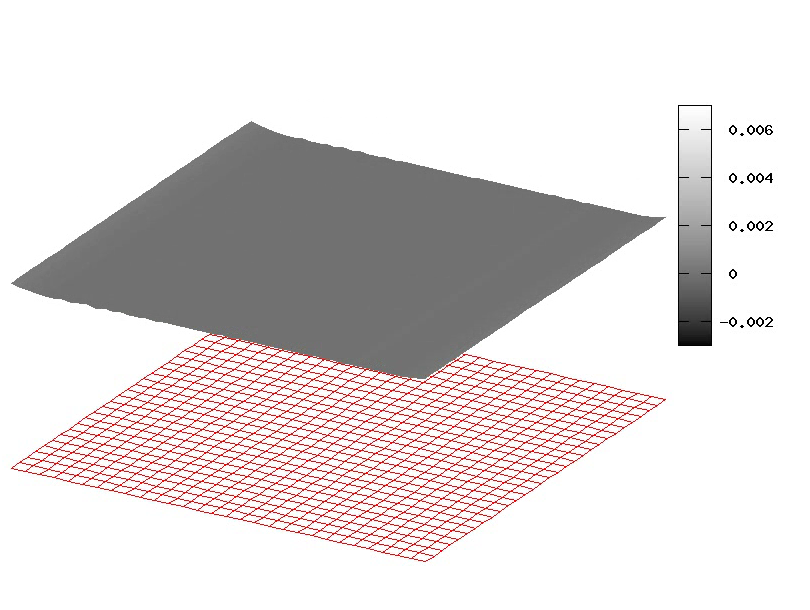
\includegraphics[width=8cm]{simple_return4.png}
    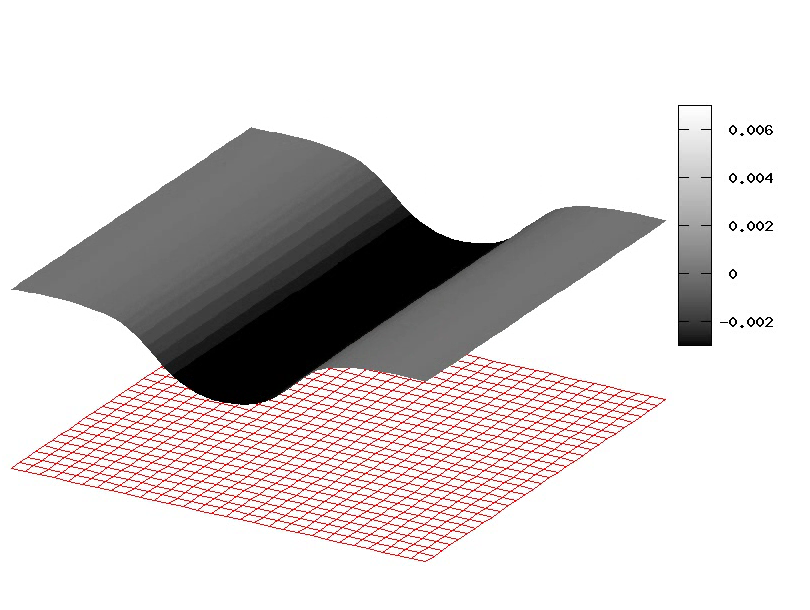
\includegraphics[width=8cm]{simple_return6.png}
    \caption{Графическое представление о возвращенной волне}
    \label{fig:ReturnWaveSmall}
\end{figure}

На рис.\ref{fig:ReturnWave} представлена динамика движения волны следующего вида $u_0=0\;v_0=0\;\eta_0=7 \cdot 10^{-3}e^{(-100 (x-0.5)^2)}$
и ее возвращения. В данном случае произошло возвращение волны с противоположной по знаку амплитуды.

\begin{table}[H]
    \label{tab:FirstResult}
    \caption{Параметры для расчетов с возвращением волны над ровным дном}
    \begin{center}
	\begin{tabular}{|c|c|c|}
	    \hline
	    Размер области & $1\times1$\\
	    \hline
	    Количество шагов & $600$\\
	    \hline
	    Шаг по времени & $0.01$\\
	    \hline
	    Шаг сетки & $0.01$\\
	    \hline
	    Точность метода & $10^{-7}$\\
	    \hline
	    Форма дна & $H(x,y)=0.01$\\
	    & $B(x,y,t)=0$\\
	    \hline
	\end{tabular}
    \end{center}
\end{table}

На рис.\ref{fig:ReturnAfterWave} представлено продолжение расчета с начальных данных, взятых после выхода волны следующего вида $u_0=0\;v_0=0\;\eta_0=7\;\cdot\;10^{-3}e^{(-100\;(x-0.3)^2)}$ из расчетой области.

\begin{table}[H]
    \label{tab:FirstResult}
    \caption{Параметры для расчетов с продолженным движением волны над ровным дном}
    \begin{center}
	\begin{tabular}{|c|c|c|}
	    \hline
	    Размер области & $1\times1$\\
	    \hline
	    Количество шагов & $300$\\
	    \hline
	    Шаг по времени & $0.001$\\
	    \hline
	    Шаг сетки & $0.01$\\
	    \hline
	    Точность метода & $10^{-7}$\\
	    \hline
	    Форма дна & $H(x,y)=0.01$\\
	    & $B(x,y,t)=0$\\
	    \hline
	\end{tabular}
    \end{center}
\end{table}

По мере исследования выяснилось, что возвращенная волна может быть в точности такой, как и изначальная, а может иметь меньшую/большую длину. Более того, задание в качестве начальных данных <<колебательного фона>> разных видов (например, произволные колебания маленькой амплитуды, либо колебания, задаваемые по определенной формуле) тоже приводит к появлению некоторых волн. Общим остается тенденция к образованию из небольшого <<колебательного фона>> волн, амплитуда которых на несколько порядков больше (в наших расчетах чаще всего на два порядка).

\newpage
\begin{figure}[H]
    \centering
    \vspace{12em}
    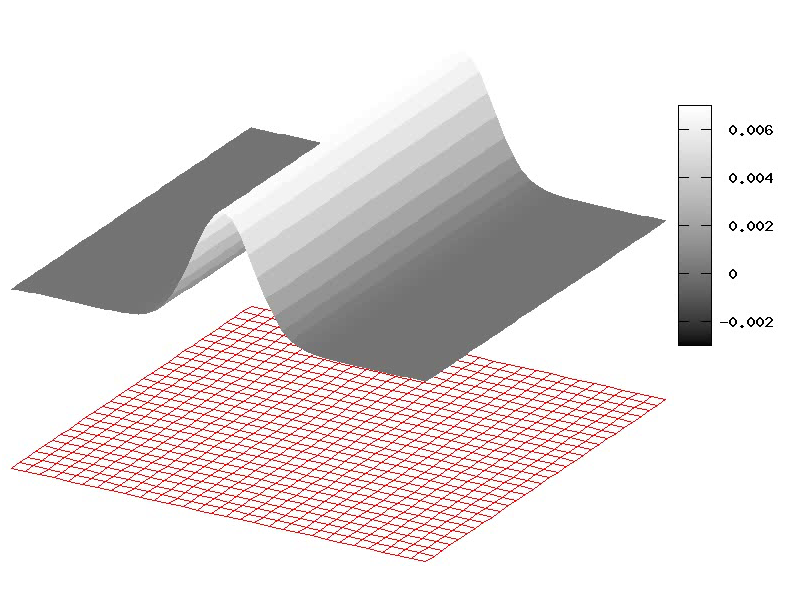
\includegraphics[width=8cm]{simple_return1.png}
    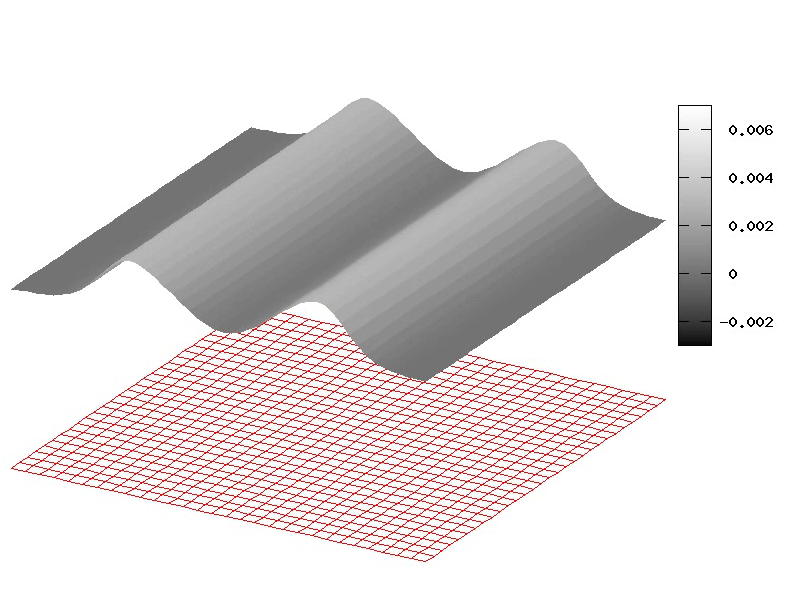
\includegraphics[width=8cm]{simple_return2.png}
    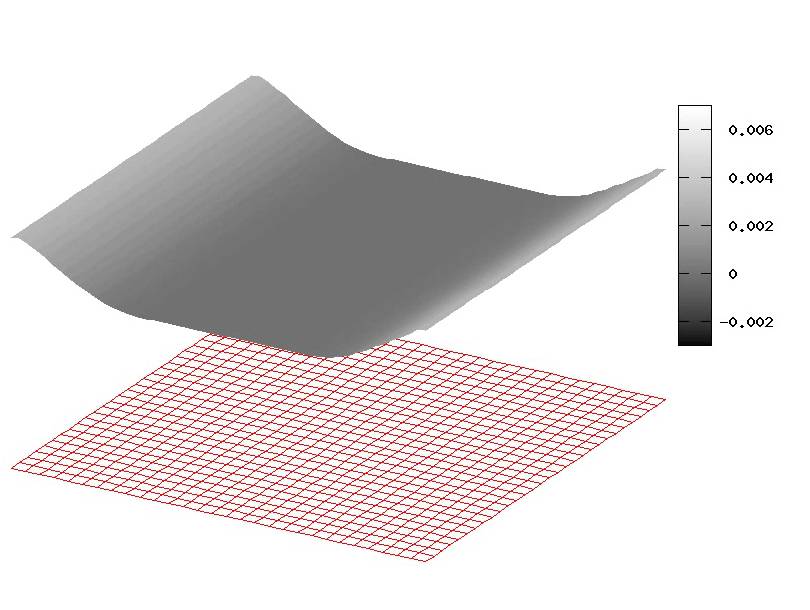
\includegraphics[width=8cm]{simple_return3.png}
    \includegraphics[width=8cm]{simple_return4.png}
    \includegraphics[width=8cm]{simple_return5.png}
    \includegraphics[width=8cm]{simple_return6.png}
    \caption{Динамика движения волны в нелинейном случае на нулевом, 80, 160, 250, 400 и 460 шагах}
    \label{fig:ReturnWave}
\end{figure}

\newpage
\begin{figure}[H]
    \centering
    \vspace{12em}
    \includegraphics[width=8cm]{return_after_wave1.png}
    \includegraphics[width=8cm]{return_after_wave2.png}
    \includegraphics[width=8cm]{return_after_wave3.png}
    \includegraphics[width=8cm]{return_after_wave4.png}
    \includegraphics[width=8cm]{return_after_wave5.png}
    \includegraphics[width=8cm]{return_after_wave6.png}
    \caption{Динамика продолженного движения волны в нелинейном случае на нулевом, 500, 1000, 1500, 2000 и 2500 шагах}
    \label{fig:ReturnAfterWave}
\end{figure}

\newpage
\addtocounter{subsection}{1}
\subsection*{Зависимость от параметров}
\addtocontents{toc}{\contentsline{subsection}{\protect\numberline{\thesubsection.}\vspace{10pt}Зависимость от параметров}{\thepage}}

Была предпринята попытка выяснить причину возникновения такого эффекта с помощью проведения серии расчетов, в которых изменялись бы основные параметры, такие как шаг по пространству, шаг по времени, точность вычислений, начальные данные, параметры, входящие в систему уравнений - т.е. глубина дна $H(x,y)$.

В таблице \ref{tab:Variables} представлены результаты расчетов и указаны следующие параметры: размер сетки, шаг по времени, соотношение $h$ к $\tau$ и результат, который может быть одним из двух - волна возвращается либо нет.

Если в таблице указаны два расчета с одинаковыми параметрами, но разным результатом, это значит, что другие параметры, не отраженные в таблице, были различными (точность вычислений, начальные данные).

\begin{table}[p]
    \caption{Результаты расчетов с различными параметрами}
    \label{tab:Variables}
    \begin{center}
	\begin{tabular}{|c|c|c|c|}
	    \hline
	    Размер сетки & Соотношение $h \tau$ & Шаг по времени & Результат\\
	    \hline
	    100x100 & $1.0101\ldots$ & 0.01 & не возвращается\\
	    \hline
	    100x100 & $1.0101\ldots$ & 0.01 & не возвращается\\
	    \hline
	    100x100 & 1.0101... & 0.01 & возвращается\\
	    \hline
	    50х50 & 20,4081632 & 0.001 & возвращается\\
	    \hline
	    50х50 & 2,04081632 & 0.01 & не возвращается\\
	    \hline
	    150х150 & 0,67114093 & 0.01 & не возвращается\\
	    \hline
	    150х150 & 0,67114093 & 0.01 & возвращается\\
	    \hline
	    100х100 & 1.0101... & 0.01 & возвращается\\
	    \hline
	    100х100 & 1.0101... & 0.01 & возвращается\\
	    \hline
	    200х200 & 0,50251256 & 0.01 & не возвращается\\
	    \hline
	    200х200 & 5,0251256 & 0.001 & возвращается\\
	    \hline
	    50х50 & 2,04081632 & 0.01 & не возвращается\\
	    \hline
	    50х50 & 20,4081632 & 0.001 & возвращается\\
	    \hline
	    50х50 & 40,963264 & 0.0005 & возвращается\\
	    \hline
	    50х50 & 20,4081632 & 0.001 & возвращается\\
	    \hline
	    50х50 & 2,04081632 & 0.01 & не возвращается\\
	    \hline
	    50х50 & 0,204081632 & 0.1 & не возвращается\\
	    \hline
	    50х50 & 40,8163264 & 0.0005 & возвращается\\
	    \hline
	    50х50 & 4,08163264 & 0.005 & возвращается\\
	    \hline
	    50х50 & 0,408163264 & 0.05 & не возвращается\\
	    \hline
	    50х50 & 0,408163264 & 0.05 & не возвращается\\
	    \hline
	    100х100 & 0,20202... & 0.05 & не возвращается\\
	    \hline
	    100х100 & 1,0101... & 0.01 & не возвращается\\
	    \hline
	    100х100 & 1,0101... & 0.01 & возвращается\\
	    \hline
	\end{tabular}
    \end{center}
\end{table}

Графическое представление этих данных дает некоторое представление о зависимостях между параметрами и результатом.
На рис.\ref{fig:VariablesGraph} изображены характеристики \nocite{yanenko} уравнения, которое описывает движение волны $\frac{\partial x}{\partial t}=g\;\frac{\partial x}{\partial t}=H $, где $H$ - постоянная часть дна (в данных расчетах $H=0.1$). На графике точками указаны проведенные расчеты, в соответствии с отношением $h$ к $\tau$ . Кругами отмечены расчеты, в которых волна возвращается, квадратами - в которых волна не возвращается.

\begin{figure}[H]
    \centering
    \includegraphics[height=8cm]{variables.png}
    \caption{Графическое представление данных о возвращении}
    \label{fig:VariablesGraph}
\end{figure}

\newpage
В результате такого представления были сделать предположение о причинах возникновения эффекта возвращения:
\begin{itemize} 
    \item если соотношение $h$ и $\tau$ больше, чем верхняя характеристика ($g$), то волна всегда возвращается.
    \item Если меньше - то возвращение зависит от других параметров.
    \item В области ниже характеристики $H$  расчетов нет, но близкие к ним (соотношение $h$ и $\tau$ примерно $0.2$) характеризуются тем, что волна в них почти никогда не возвращается. Помимо этого можно отметить тот факт, что в тех расчетах, где волна возвращалась, при увеличении $H$ волна переставала возвращаться. В связи с этим можно предположить, что все расчеты, соотношение $h$ и $\tau$ в которых меньше нижней характеристики ($H$), характеризуются тем, что волна не возвращается
\end{itemize}

\addtocounter{subsection}{1}
\subsection*{Расчет с начальных данных}
\addtocontents{toc}{\contentsline{subsection}{\protect\numberline{\thesubsection.}\vspace{10pt}Расчет с начальных данных}{\thepage}}

В качестве интересного результата были получены начальные данные небольшой <<нулевой>> амплитуды, при подстановке которых в расчет наблюдается появление движущейся в области волны. Т.о. более правильно говорить не о <<возвращении>>, а о <<возникновении>> волны на поверхности жидкости, что приводит к мысли о возможности моделирования такого явления, как <<волна-убийца>>.

\begin{table}[H]
    \label{tab:FirstResult}
    \caption{Параметры для расчетов с возникновением волны}
    \begin{center}
	\begin{tabular}{|c|c|c|}
	    \hline
	    Размер области & $1\times1$\\
	    \hline
	    Количество шагов & $2000$\\
	    \hline
	    Шаг по времени & $0.001$\\
	    \hline
	    Шаг сетки & $0.01$\\
	    \hline
	    Точность метода & $10^{-4}$\\
	    \hline
	    Форма дна & $H(x,y)=0.1\;B(x,y,t)=0$\\
	    \hline
	\end{tabular}
    \end{center}
\end{table}

На рис.\ref{fig:ReturnMoveWave} представлена динамика движения такой волны.

\newpage
\begin{figure}[H]
    \centering
    \vspace{12em}
    \includegraphics[width=8cm,trim=0 4mm 0 0,clip]{return_move_wave1.png}
    \includegraphics[width=8cm,trim=0 4mm 0 0,clip]{return_move_wave2.png}
    \includegraphics[width=8cm,trim=0 4mm 0 0,clip]{return_move_wave3.png}
    \includegraphics[width=8cm,trim=0 4mm 0 0,clip]{return_move_wave4.png}
    \caption{Движение волны с <<нулевого фона>> на 200, 700, 1200 и 1600 шагах}
    \label{fig:ReturnMoveWave}
\end{figure}

\newpage
\addtocounter{section}{1}
\setcounter{subsection}{0}
\setcounter{equation}{0}
\section*{Выводы} 
\addtocontents{toc}{\contentsline{section}{\protect\numberline{\S\;\thesection.}\vspace{10pt}Выводы}{\thepage}}

Проанализировав представленные расчеты, можно сделать несколько выводов:
\begin{itemize}
    \item Предлагаемый подход к решению задачи (\ref{eq:MainVectorForm})-(\ref{eq:BoundaryCondition}) с использованием неявных схем и аппроксимации исходной системы уравнений на границе конечной области позволяет находить в ней решение без отражений или искажений. Для всех случаев (сложная начальная форма свобожной поверхности, неровное дно, линейная и нелинейная форма уравнения) было получено решение, соответствующее реальным физическим представлениям о задаче, возмущения свободной поверхности безпрепятственно выходили из области, при этом не искажаясь и не порождая отражений.
    \item Расчет в линейном и нелинейном случае показал, что нелинейная форма уравнений (\ref{eq:MainVectorForm})-(\ref{eq:BoundaryCondition}) приводит к тому, что волны свободной поверхности со временем меняют свою форму, становятся менее симметричными относительно своего центра.
	\begin{figure}[H]
	    \centering
	    \includegraphics[width=8cm]{Lin.png}
	    \includegraphics[width=8cm]{Nonlin.png}
	    \caption{Форма волны в линейном(слева) и нелинейном(справа) случае}
	    \label{fig:Lin_Nonlin_Wave}
	\end{figure}
	Для нелинейных уравнений за основной волной формируются вторичные колебания, амплитуда которых много меньше исходной. При этом указанные эффекты со временем проявляются все более сильно.
\end{itemize}